\documentclass[12pt]{report}
\usepackage{graphicx}
\usepackage{caption}
\usepackage[english]{babel}
\usepackage{caption}
\usepackage{capt-of}
\usepackage{color, colortbl}
\usepackage[hidelinks]{hyperref}
\usepackage[numbers]{natbib}
\usepackage[nohyperlinks, printonlyused, withpage, smaller]{acronym}
\usepackage[ngerman]{datetime}
\usepackage{chngcntr}
\usepackage{pdfpages}
\usepackage{enumitem}
\usepackage{amsmath}
\usepackage{tikz}
\usepackage[skins]{tcolorbox}
\usepackage{rotating}
\usepackage{framed}
\counterwithin{figure}{section}
\usepackage{lipsum}
\usepackage{float}
\usepackage{listings}
\usepackage{xcolor}
\usepackage{listing}
\usepackage{hyperref}
\usepackage{lscape}
\usepackage{longtable}

\def\frontmatter{%
    \pagenumbering{roman}
    \setcounter{page}{1}
    \renewcommand{\thesection}{\Roman{section}}
}%

\def\mainmatter{%
    \pagenumbering{arabic}
    \setcounter{page}{1}
    \setcounter{section}{0}
    \renewcommand{\thesection}{\arabic{section}}
}%

\def\backmatter{%
    \setcounter{section}{0}
    \renewcommand{\thesection}{\Alph{section}}
}%
\renewcommand{\listfigurename}{\begingroup
    \tocchapter{}
    \tocfile{\listoffigurename}{B Illustration Directory}
\endgroup}

\begin{document}
\frontmatter

\begin{titlepage}
    \newcommand{\HRule}{\rule{\linewidth}{1.5mm}}
    \center{}
    \begin{figure}
        \centering
        
\includegraphics[width=0.5\textwidth]{img/hslogo}\label{pic:Logo}
    \end{figure}

    \begin{center}
    \end{center}

    {\huge Masterproject}\\[0.4cm]
    \begin{center}
    \end{center}
    {\Large Data Science }\\
    {Analytics and Prediction for Rental Bike Usage in London}
    \vfill
    \begin{center}
        {Contributors:}\ \\
        \vspace{0.25\baselineskip}
        {\Large Anass Khaldi, Guillaume Goni, Kathi Rodi, Pascal Riedel}
    \end{center}
    \vfill
    \begin{center}
        {\large Expert: Prof.\ Dr.\ von Schwerin }\\
    \end{center}
    \begin{center}
        {\large Expert: Prof.\ Dr.\ Herbort}
    \end{center}
    \begin{center}
        {\large Expert: Prof.\ Dr.\ Goldstein}
    \end{center}
    \vfill
    {\Large \today}

\end{titlepage}

\newpage
\tableofcontents
\mainmatter{}
\newpage
\chapter{Project Presentation and Organization}
% TODO: reorganize, rewrite
% vim:ft=tex

\section{Introduction}

No matter in which area you move there is a huge chance that data science will be there too. It is one of the fast moving trends during the last years which is caused by the unimaginable amount of data we produce everyday. We could gain a lot of knowledge out of this data, but therefore we must analyze it. That is when data science comes into play. But with the help of data science we can not just analyze the past we can also predict the future.\\\\
Let's say we have a bike rental station which provides to rent bikes for a certain amount of time. We track the duration of the rental, the time of rental, the routes the bikes rode and lot more information. By processing all this data it is possible to predict the future usage of the bikes and the most frequented routes to specific times.
That is what the main goal of this project represents. This project report deals with tasks which can be summarized by \emph{preparatory steps} to reach this final goal. The project duration is divided into two semesters. The tasks of the first part will be discussed in this paper.


% vim:ft=tex

\section{Task Description}\label{tasks}

The first part can be roughly divided into two parts:
\begin{enumerate}
\item Data Engineering
\begin{itemize}
\item Data Profiling
\item identify potential difficulties
\item store data set
\end{itemize}
\item Virtual Infrastructure
\begin{itemize}
\item install and configure Nominatim
\item install and evaluate different Hadoop distributions
\end{itemize}
\end{enumerate}
The project should be implemented in an agile manner, therefore we will follow the development process of \textbf{Scrum}. This allows flexibility during the project in terms of specific tasks and topics.
\\\\
To gain a better understanding of the project and its goals we created a \glqq Big Picture\grqq of the applied technologies and the relations among themselves which can be seen in figure \ref{fig:big}.

\begin{figure}[H]
\hspace{-0.9cm}
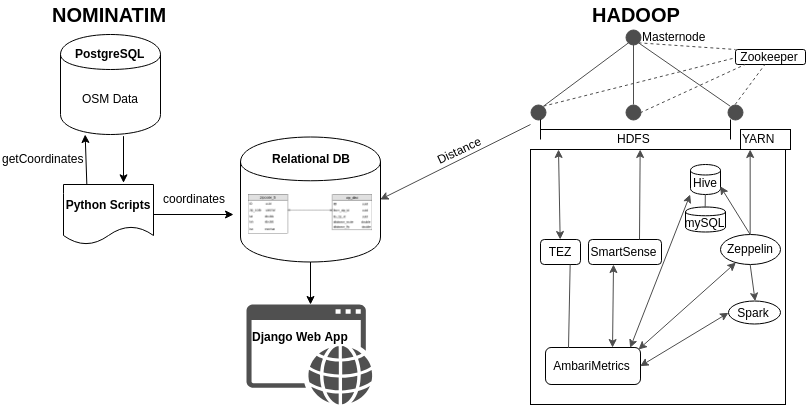
\includegraphics[width=1.1\textwidth]{img/big}
\captionof{figure}{Overview of project architecture}\label{fig:big}
\end{figure}
\noindent According to this picture the project can be classified more detailed into four parts:
\begin{enumerate}
\item Nominatim
\item Hadoop
\item Database
\item WebApp
\end{enumerate}
The implementation of those four parts will be documented in the following chapters.

% vim:ft=tex

\section{Task Description (Semester 2)}
The first part of the second semester is dedicated to finish the remaining tasks of the previous semester. This includes finish the Django Web Application as well as implementing an appropriate algorithm to fill the distance database.\\\\
Moreover the actual goal of the second semester is to implement prediction algorithms in order to forecast the usage of rental bikes in London on a daily as well as on a hourly base. Therefore data profiling tasks need to be done in order to investigate the provided data. Furthermore additional features like weather data should be researched and prepared to be added to the feature matrix. At the same time several algorithms need to be tested to find out the best fitting one to our needs. For this purpose two different libraries (Scikit-Learn and Spark) should be analyzed and tested.\\
A big part depicts of the data profiling part where data should be processed for further prediction usage. This includes data cleansing as well as data preparation. Once the data is ready a model can be implemented and first predictions can be made on a daily base. After that, the algorithms need to be evaluated and improved. In order to do so a suitable rating as well as meaningful plots need to be found, to get a better idea of the prediction results. \\
Moreover the same need to be done for the prediction on a hourly base. Which also needs specific data preparation steps.\\
After first predictions the features should be evaluated to gain more knowledge of which features are meaningless and which improve the prediction accuracy. A Further task is to find proper additional features which could also improve the prediction. Therefore research need to be done as well as further data preparation steps and evaluation tasks.\\\\
Another goal is to configure a Hadoop Cluster at University which should provide more computing capacity in order to make predictions out of very large data sets.

% vim:ft=tex

\section{Collaboration Technologies}

Since we want to ensure efficiency which includes that everyone has access to required data, can exchange data and that data can be versioned,  we decided to work with several technologies which will be explained further in the following sections.
\subsection{IceScrum}
As mentioned in the chapter before the development process should be done by using Scrum methods.
Those methods includes \emph{Sprint Plannings, Daily Scrums, Retrospectives} and \emph{Sprint Reviews}.
To apply the methods properly it was very helpful to use \emph{IceScrum} which is a web application in order to use Scrum. It provides storyboards on which tasks can be accepted. Furthermore it helps to keep track of progress and remaining tasks by burndowncharts as well as reports. We used IceScrum mainly for the sprint planning. To be precise for writing, estimating, prioritizing tasks, maintain our backlog and to distribute the incurred tasks as well as keeping track of our remaining story points and our progress.
\\IceScrum offers furthermore different roles which should be satisfied in Scrum. 
There is the \emph{Team} which is responsible to deliver the committed delivery in time and with the defined quality. In our case the Team consists of Anass Khaldi, Guillaume Goni and Pascal Riedel. Within the team there is one \emph{Scrum Master}, this role was taken by Kathi Rodi. The Scrum Master is responsible to ensure the team keeps to the values and practices of Scrum, sort of like a coach. He  removes impediments, facilitates meetings and work with product owners as well. This leads us to the next role in Scrum the \emph{Product Owner} which is the project`s key stakeholder. The Product Owner does not get to determine how much work happens in the sprint cycles, or alter the goals for that sprint. Product Owners must be available to the team, and engage actively with it. In this project the Product Owners are Prof. Dr. von Schwerin, Prof. Dr. Herbort and Prof. Dr. Goldstein.
\subsection{Box}
Besides IceScrum we also used \emph{Box} for collaborating.  Our Box includes for example the documentation of our daily scrums. We created a template which is used to log every daily meeting. According burndowncharts and reports will be stored there as well. Furthermore we used the box for recording our working hours and to exchange documents.
\subsection{GitHub}
To group our code base and have versioned on it, we created a GitHub account which is available at 
\href{https://github.com/dataBikeHsUlm}{https://github.com/dataBikeHsUlm}.
For the sake of clarity we created three repositories ordered by the main topics:
\begin{itemize}
\item WebApp: for the web server
\item NominatimLibrary: for the Jupyter notebooks
\item MapReduce: for the scripts for Hadoop
\end{itemize}
\subsection{Skype}
We carried out our daily scrums every monday at 4 pm as well as every thursday at 1.30 pm. On thursdays we have lectures together the whole day, hence the daily scrums on thursdays takes place at the university. Since it wasn't`t possible for the whole team to meet mondays as well, we decided to hold those daily scrums via Skype.

% vim:ft=tex

\section{Responsibilities}

\subsection{First semester}

Within Scrum the team is self-organizing and cross-functional. This means that every
team member can choose tasks fitting his knowledge base as well as his preferences
and interests. Hence everyone was free to suggest and accept the tasks he liked
most.
It turned out that the team leads a very good self-organization because
everyone of us has a specific interest and knowledge according to the tasks of
the project.
Therefore Anass Khaldi was responsible to install the Nominatim server
and it's components. In the second sprint his main part was to research Django
and how we can display maps on our web application. In the third sprint it was
his responsibility to install graphhopper and to fix the according issues as well
as issues of Hadoop.
The main part of the Jupyter notebook to research nominatim functions like compute
centroids, compute distances by route and doing all in bulk was done by Guillaume
Goni. In the second sprint he created all GitHub repositories for storing our work.
He wrote the script to initialize the database as well as the one to fill the database.
Therefore he researched for best ways to collect zip codes and find the solution
in the PostgresDB.\@
Moreover he prepared a tutorial about Django for the rest of the team members.
As mentioned before Kathi Rodi took over the role of the Scrum Master, hence it
was her responsibility to ensure that the scrum artifacts were kept as well as
correspond with the Product Owners. Apart from her tasks as a Scrum Master she
was responsible to provide a box for collaborating with all needed documents like
templates for daily scrums, sprint plannings, reviews, retrospectives and tracking
the working hours. Furthermore she created the presentation for every sprint.
Moreover she solved several tasks like create Jupyter notebooks for geocode,
reverse geocoding and compute distances as the crow flies, create the ER model,
install the MySQL database and to research for Graphhopper.
In the end it was her responsibility to write a project report and add the task
descriptions of the team members to it.\\Pascal Riedel was responsible for research,
document and compare the different Hadoop distributions. With the help of his
weightened comparison table we could take the decision for one specific distribution.
It was also his part to install the \acs{hdp} as well as to implement a Map Reduce job.
During the first project phase he solved several issues according to \acs{hdp}.
Furthermore he was responsible for the data profiling part and to create associated
Zepellin notebooks.
% For more details please have a look at the responsibility table which could be
% found in attachment~\ref{resp}.

\subsection{Second semester}

GG:
postcodes db + 2-digits distances db + implementation in Django
learning/prediction on hourly data
features for all stations
pandas profiling
% help organisation of report and presentation

Kathi:
Scrum Master: presentations/reports + meetings organisation + sprint planning + ...
created view for Django app

Pascal Riedel continued taking care of Hadoop by fixing running issues on our
cluster and by setting up another one on dedicated machines.
He also worked on the management of the Nominatim server by cleaning the Nominatim
PostgreSQL database to import only Europe data and configured Apache to run with
Django, so Django doesn't run in develop mode any more.
Finally on the configuration part, he fixed Graphhopper, finished preparing it
and worked on an API to use it effectively. For these tasks, he was helped by
Anass Khaldi.  
This done, he could research a better analysis on the bike rental on the whole
London network with a map of all the stations and the paths used by the users.
Pascal used PySpark on the Hadoop cluster to prepare the raw bike rental dataset
for prediction. He first prepared a daily-based dataset joined with weather usage
and holidays, and later worked on a hourly-based one.

Kathi Rodi and Anass Khaldi mainly worked on the data learning and prediction
parts. They prepared the data and researched different learning algorithms with
different parameters for a more accurate prediction. They also investigated the
relevance of the different features and better ways to measure accuracies.
Kathi also extracted and prepared extra features that could be added to the
dataset to improve it (demographic data, events, income and political opinions).
Guillaume Goni finished preparing and parsing these new features and integrating
them into our existing datasets.

% vim:ft=tex

\section{Conclusion}

\chapter{Postal Code Database (Nominatim and Graphhopper)}
% vim:ft=tex

\section{Nominatim}
Nominatim is a tool to search \ac{osm} data by name and address and to generate
synthetic addresses of OSM points (reverse geocoding).
Nominatim provides geocoding based on OpenStreetMap data. It uses a PostgreSQL
database as a backend for storing the data.
There are three basic parts to Nominatim's architecture: the data import, the address
computation and the search frontend.
The data import stage reads the raw OSM data and extracts all information that is useful
for geocoding. This part is done by \textbf{osm2pgsql}, the same tool that can also be used to
import a rendering database. It uses the special gazetteer output plugin in \textbf{osm2pgsql/output-gazetter.[ch]pp}. The result of the import can be found in the database table \textbf{place}.
The address computation or indexing stage takes the data from \textbf{place} and adds
additional information needed for geocoding. It ranks the places by importance, links
objects that belong together and computes addresses and the search index. Most of
this work is done in \ac{pl} via database triggers and can be found in the file \textbf{sql/
functions.sql}.\\
The search frontend implements the actual API. It takes queries for search and reverse
geocoding queries from the user, looks up the data and returns the results in the requested
format. This part is written in php and can be found in the \textbf{lib/} and \textbf{website/} directories.\\
When we received the Nominatim server, we created the non-administrator user account for our use and we added the SSH public keys of all the team members.
\subsection{Installation}
These instructions expect that you have a freshly installed Ubuntu 18.04.
Make sure all packages are are up-to-date by running:
\begin{lstlisting}[language=bash,breaklines=true]
sudo apt-get update -qq
\end{lstlisting}
Now you can install all packages needed for Nominatim:
\begin{lstlisting}[language=bash,breaklines=true]
sudo apt-get install -y build-essential cmake g++ libboost-dev libboost-system-dev \
libboost-filesystem-dev libexpat1-dev zlib1g-dev libxml2-dev\
libbz2-dev libpq-dev libproj-dev \
postgresql-server-dev-10 postgresql-10-postgis-2.4 \
postgresql-contrib-10 \
apache2 php php-pgsql libapache2-mod-php php-pear php-db \
php-intl git
\end{lstlisting}
If you want to run the test suite, you need to install the following additional packages:
\begin{lstlisting}[language=bash,breaklines=true]
sudo apt-get install -y python3-setuptools python3-dev python3-pip \
python3-psycopg2 python3-tidylib phpunit php-cgi
pip3 install --user behave nose
sudo pear install PHP_CodeSniffer
\end{lstlisting}
\subsubsection{System Configuration}
The following steps are meant to configure a fresh Ubuntu installation for use with Nominatim.
You may skip some of the steps if you have your OS already configured.
Nominatim will run as a global service on your machine. It is therefore best to install it under its
own separate user account. In the following we assume this user is called \textbf{nominatim} and the
installation will be in \textbf{/srv/nominatim}. To create the user and directory run:
\begin{lstlisting}[language=bash,breaklines=true]
sudo useradd -d /srv/nominatim -s /bin/bash -m nominatim
\end{lstlisting}
You may find a more suitable location if you wish.
To be able to copy and paste instructions from this manual, export user name and home
directory now like this:
\begin{lstlisting}[language=bash,breaklines=true]
export USERNAME=nominatim
export USERHOME=/srv/nominatim
\end{lstlisting}
Never, ever run the installation as a root user.
Make sure that system servers can read from the home directory:
\begin{lstlisting}[language=bash,breaklines=true]
chmod a+x $USERHOME
\end{lstlisting}
\subsubsection{Setting up PostgreSQL}
Tune the PostgreSQL configuration, which is located in\\ \textbf{/etc/postgresql/9.5/main/postgresql.conf}. You might want to tune your PostgreSQL installation so that the later steps make best use of your hardware. You should tune the following parameters in your \textbf{postgresql.conf} file.
\begin{lstlisting}[language=bash,breaklines=true]
shared_buffers (2GB)
maintenance_work_mem (10GB)
work_mem (50MB)
effective_cache_size (24GB)
synchronous_commit = off
checkpoint_segments = 100 # only for postgresql <= 9.4
checkpoint_timeout = 10min
checkpoint_completion_target = 0.9
\end{lstlisting}
The numbers in brackets behind some parameters seem to work fine for 32GB RAM machine.
Adjust to your setup.
For the initial import, you should also set:
\begin{lstlisting}[language=bash,breaklines=true]
fsync = off
full_page_writes = off
\end{lstlisting}
Don't forget to reenable them after the initial import or you risk database corruption.
\textbf{Autovacuum} must not be switched off because it ensures that the tables are frequently
analyzed.
\subsubsection{Setting up the Webserver}
The \textbf{website} directory in the \textbf{build} directory contains the configured website. Include the directory into your web browser to serve php files from there.\\
Make sure your Apache configuration contains the required permissions for the directory and
create an alias:
\begin{lstlisting}[language=bash,breaklines=true]
<Directory "/srv/nominatim/build/website">
Options FollowSymLinks MultiViews
AddType text/html
.php
DirectoryIndex search.php
Require all granted
</Directory>
Alias /nominatim /srv/nominatim/build/website
\end{lstlisting}
The path of the build directory (\textbf{/srv/nominatim/build}) should be replaced with the location of your build directory. After making changes in the apache config you need to restart apache. The website should now be available on http://localhost/nominatim.
Restart the PostgreSQL service after updating this config file.
\begin{lstlisting}[language=bash,breaklines=true]
sudo systemctl restart postgresql
\end{lstlisting}
Finally, we need to add two PostgreSQL users: one for the user that does the import and another
for the webserver which should access the database for reading only:
\begin{lstlisting}[language=bash,breaklines=true]
sudo -u postgres createuser -s $USERNAME
sudo -u postgres createuser www-data
\end{lstlisting}
You need to create an alias to the website directory in your apache configuration. Add a
separate nominatim configuration to your webserver:
\begin{lstlisting}[language=bash,breaklines=true]
sudo tee /etc/apache2/conf-available/nominatim.conf << EOFAPACHECONF
<Directory "$USERHOME/Nominatim/build/website">
Options FollowSymLinks MultiViews
AddType text/html
.php
DirectoryIndex search.php
Require all granted</Directory>
Alias /nominatim $USERHOME/Nominatim/build/website
EOFAPACHECONF
\end{lstlisting}
Then enable the configuration and restart apache:
\begin{lstlisting}[language=bash,breaklines=true]
sudo a2enconf nominatim
sudo systemctl restart apache2
\end{lstlisting}
\subsubsection{Building and Configuration}
Get the source code for the release and change into the source directory:
\begin{lstlisting}[language=bash,breaklines=true]
cd $USERHOME
wget https://nominatim.org/release/Nominatim-3.2.0.tar.bz2
tar xf Nominatim-3.2.0.tar.bz2
cd Nominatim-3.2.0
\end{lstlisting}
The code must be built in a separate directory. Create this directory, then configure and build
Nominatim in there:
\begin{lstlisting}[language=bash,breaklines=true]
mkdir build
cd build
cmake ..
make
\end{lstlisting}
You need to create a minimal configuration file that tells nominatim where it is located on the
webserver:
\begin{lstlisting}[language=bash,breaklines=true]
tee settings/local.php << EOF
<?php
@define('CONST_Website_BaseURL', '/nominatim/');
EOF
\end{lstlisting}
After those steps Nominatim is ready to use.
\subsection{Database import}
The following instructions explain how to create a Nominatim database from an OSM planet file
and how to keep the database up to date. It is assumed that the Nominatim software itself is already successfully installed.
\subsubsection{Flatnode files}
If you plan to import a large dataset (e.g. Europe, North America, planet), you should also
enable flatnode storage of node locations. With this setting enabled, node coordinates are
stored in a simple file instead of the database. This will save you import time and disk storage.
Add to your settings/local.php:
\begin{lstlisting}[language=bash,breaklines=true]
@define('CONST_Osm2pgsql_Flatnode_File', '/path/to/flatnode.file');
\end{lstlisting}
Replace the second part with a suitable path on your system and make sure the directory exists.
There should be at least 40GB of free space.
\subsubsection{Initial import of the data}
Important: first try the import with a small excerpt, for example from \textbf{Geofabrik}.
Download the data to import and load the data with the following command:
\begin{lstlisting}[language=bash,breaklines=true]
./utils/setup.php --osm-file <data file> --all [--osm2pgsql-cache 28000] 2>&1 | tee setup.log
\end{lstlisting}
The \textbf{--osm2pgsql-cache} parameter is optional but strongly recommended for planet imports. It
sets the node cache size for the \textbf{osm2pgsql} import part (see -C parameter in osm2pgsql help).
As a rule of thumb, this should be about the same size as the file you are importing but never
more than 2/3 of RAM available. If your machine starts swapping reduce the size.
Computing word frequency for search terms can improve the performance of forward geocoding
in particular under high load as it helps PostgreSQL' query planner to make the right decisions. To
recompute word counts run:
\begin{lstlisting}[language=bash,breaklines=true]
./utils/update.php --recompute-word-counts
\end{lstlisting}
This will take a couple of hours for a full planet installation. You can also defer that step to a
later point in time when you realise that performance becomes an issue. Just make sure that
updates are stopped before running this function.
\subsubsection{Updating the data}
There are many different possibilities to update the Nominatim database. The following section
describes how to keep it up-to-date with \textbf{Pyosmium}. For a list of other methods see the output of
\textbf{./utils/update.php --help}. It is recommended to install Pyosmium via pip. Run (as the same user who will later run the updates):
\begin{lstlisting}[language=bash,breaklines=true]
pip install --user osmium
\end{lstlisting}
Nominatim needs a tool called \textbf{pyosmium-get-updates}, which comes with Pyosmium. You need
to tell Nominatim where to find it. Add the following line to your \textbf{settings/local.php}:
\begin{lstlisting}[language=bash,breaklines=true]
@define('CONST_Pyosmium_Binary', '/home/user/.local/bin/pyosmium-get-changes');
\end{lstlisting}
The path above is fine if you used the \textbf{--user} parameter with pip. Replace user with your user
name. \\
Next the update needs to be initialised. By default Nominatim is configured to update using the
global minutely diffs. If you want a different update source you will need to add some settings to \textbf{settings/local.php}.
For example, to use the daily country extracts diffs for Ireland from geofabrik add the following:
\begin{lstlisting}[language=bash,breaklines=true]
// base URL of the replication service
@define('CONST_Replication_Url', 'https://download.geofabrik.de/europe/ireland-and-northern-
ireland-updates');
// How often upstream publishes diffs
@define('CONST_Replication_Update_Interval', '86400');
// How long to sleep if no update found yet
@define('CONST_Replication_Recheck_Interval', '900');
\end{lstlisting}
To set up the update process now run the following command:
\begin{lstlisting}[language=bash,breaklines=true]
./utils/update.php --init-updates
\end{lstlisting}
It outputs the date where updates will start. Recheck that this date is what you expect.
The \textbf{--init-updates} command needs to be rerun whenever the replication service is changed.\\
The following command will keep your database constantly up to date:
\begin{lstlisting}[language=bash,breaklines=true]
./utils/update.php --import-osmosis-all
\end{lstlisting}
Note that even though the old name \glqq import-osmosis-all\grqq has been kept for compatibility
reasons, Osmosis is not required to run this - it uses Pyosmium behind the scenes.\\
Nominatim will response with the following data formats:
\begin{itemize}
\item JSON
\item JSONv2
\item GeoJSON
\item Geocode JSON
\item XML
\end{itemize}
\subsection{Usage}
As we want to use python for working with Nominatim we use the python package \textbf{geopy} to interact with the server. \\
Up to now, we were using the default public Nominatim server \citep{Nominatim2019}. As we want to use our own Nominatim server we researched for connecting the geopy library to it.\\
First, the Nominatim server needed to be configured with Apache, the configuration that was done earlier
wasn't working properly so we firstly had to fix that. The server can be accessed at the following url: \href{http://i-nominatim-01.informatik.hs-ulm.de/nominatim/}{http://i-nominatim-01.informatik.hs-ulm.de/nominatim/}.\\
After that  HTTPS isn't enabled on the server. Of course, we can set it up later but for now we need to disable it for geopy, it is done by setting:
\begin{lstlisting}[language=bash,breaklines=true]
geopy.geocoders.options.default_scheme = "http"
\end{lstlisting}
Third, our server is not very powerful and being quite new, it has not cached enough queries. This can make some queries take a long time to complete and according to that the geopy query timeouts. Therefore we had to increase this limit. The final connection is shown in figure \ref{fig:con}.
\begin{figure}[H]
\hspace{2.2cm}
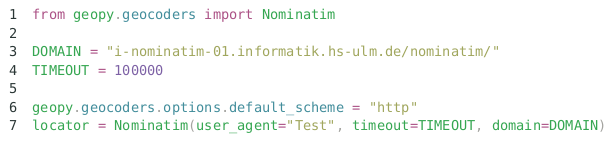
\includegraphics[width=0.8\textwidth]{img/con}\label{fig:con}
\captionof{figure}{Connection of Nominatim with geopy}\label{fig:con}
\end{figure}
\subsection{Notebooks}
In attempt to gain more knowledge on how it is possible to work with Nominatim in python we created several Jupyter notebooks. The different methods we need on the Nominatim API are grouped in a python library on the project's GitHub repository which can be accessed under\\ \href{https://github.com/dataBikeHsUlm/NominatimLibrary}{https://github.com/dataBikeHsUlm/NominatimLibrary}.
It needs \textbf{geopy} as a dependency and \textbf{osmapi} for \textbf{pyroutelib2} which can be installed via \textbf{pip}:
\begin{lstlisting}[language=bash,breaklines=true]
pip3 install geopy osmapi
\end{lstlisting}
\subsubsection{Geocoding}
Geocoding an adress means we input an adress and as an output we expect the corresponding coordinates. Therefore we have to extract the coordinates as follows:
\begin{lstlisting}[breaklines=true]
def locate (address):
    """Gets the coordinates to a given address
        
        Args: 
            address(str): String List of following arguments:house_number,road, town, city, county, state_district, state, postcode, country, country_code
	        
        Returns: 
            Associated address and coordinates 
   """
    location = geolocator.geocode(address)
    print(location.address)
    print(location.latitude, location.longitude)
\end{lstlisting}
We could also extract coordinates not by searching for a whole adress but by postalcodes:
\begin{lstlisting}[breaklines=true]
def locateCords(postcode):
    """Gets the coordinates to a given address
        
        Args: 
            postalcode(str): String of postalcode
	        
        Returns: 
            Associated coordinates as latitude and longitude
   """
    location = geolocator.geocode(postcode)
    lat = location.latitude
    lon = location.longitude
    print"The Latitude of ",postcode," is: ",lat," the Longitude is ",lon
    return (lat,lon)
\end{lstlisting}
The results are the corresponding coordinates.
\subsubsection{Reverse Geocoding}
Vice versa we can apply reverse geocoding to compute the corresponding address to given coordinates.
\begin{lstlisting}[breaklines=true]
def reverseLocate (coordinates):
    """Gets the address to given coordinates
        
        Args: 
            coordinatates(str): String List of coordinates
	        
        Returns: 
            Associated address  
    """
    location = geolocator.reverse(coordinates)
    print(location.address)
\end{lstlisting}
The result was compared with Google Maps which is shown in figure \ref{fig:geocode}.
\begin{figure}[H]
\hspace{-1.2cm}
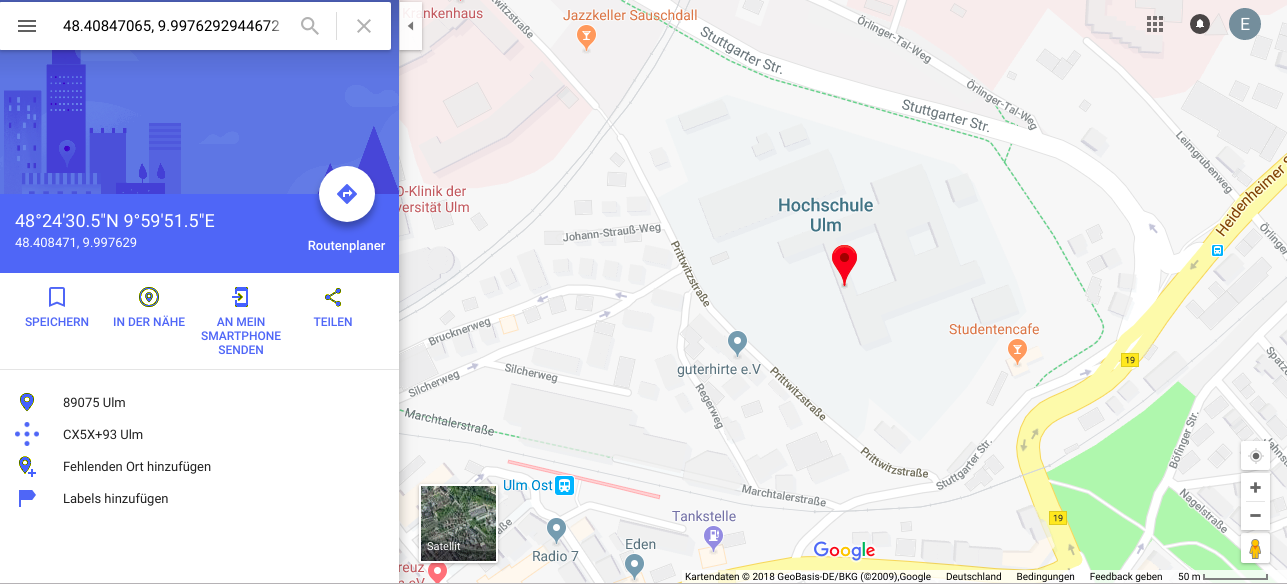
\includegraphics[width=1.2\textwidth]{img/geocode}
\captionof{figure}{Reverse Geocoding}\label{fig:geocode}
\end{figure}
\subsubsection{Querying Centroids}
As already mentioned geopy offers methods to access addresses and coordinates. We used this as follows for querying centroids:
\begin{lstlisting}[breaklines=true]
location = locator.geocode("Baden-Wuerttemberg, Deutschland")
print(location.address)
print(location.latitude, location.longitude)
\end{lstlisting}
We received the following result:
\begin{lstlisting}[language=bash,breaklines=true]
Baden-Wuerttemberg, Deutschland
48.6296972 9.1949534
\end{lstlisting}
We entered the given coordinates for the centroid of Baden-Wuerttemberg (\textbf{48.6296972, 9.1949534}) in Google Maps and made a route between this centroid and the one given by Google Maps as is shown in figure \ref{fig:centroid}.
\begin{figure}[H]
%\hspace{0.7cm}
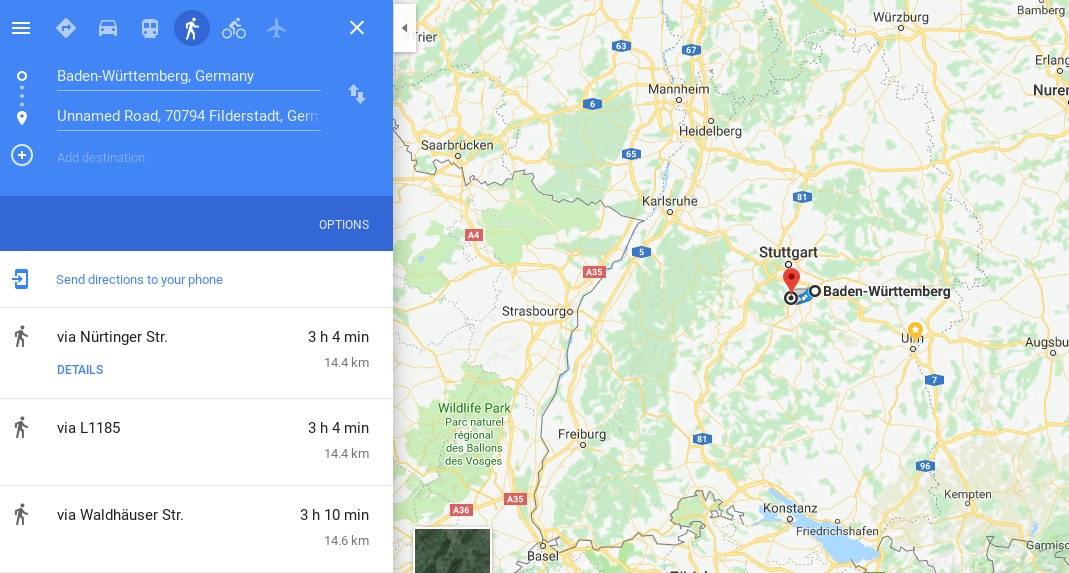
\includegraphics[width=1.0\textwidth]{img/centroid}
\captionof{figure}{Centroid of Baden-Wuerttemberg shown in Google Maps}\label{fig:centroid}
\end{figure}
We can see that there is only 14.4km between the two points. If we consider Baden-Wuerttemberg is roughly
200km wide, we have a difference of 7.2\%.
The values used here are obviously not very accurate but we can still see that the given centroid is located roughly in the center of the requested region.
The difference with Google Maps can maybe be explained by a difference of precision in the borders.
\subsubsection{Distances as the crow flies}
To compute the distance between two locations as the crow flies we can use the \textbf{distance()} method which is provided by geopy.  Therefore we have to transfer coordinates into points:
\begin{lstlisting}[breaklines=true]
def locatePoint (postcode):
    """Gets the coordinates to a given address
        
        Args: 
            postalcode(str): String of postalcode
	        
        Returns: 
            Associated coordinates as a Point
   """
    location = geolocator.geocode(postcode)
    lat = location.latitude
    lon = location.longitude
    p = location.point
    return p
locatePoint("80336")
\end{lstlisting}
Subsequently we can compute the associated routes:
\begin{lstlisting}[breaklines=true]
def getDistance(start, end):
    """Get distance of two postalcodes
        
        Args: 
            start(str): String of start postalcodes
            end (str): String of end postalcode
	        
        Returns: 
            Distance in km 
   """
    a = locatePoint(start)
    b = locatePoint(end)
    d =distance.distance(a,b).km
    print"The distance between Ulm and Munich is: ",d," km"
    return d
    
getDistance("89075","80336")
\end{lstlisting}
The result was compared to Google Maps and can be seen in figure \ref{fig:fly}.
\begin{figure}[H]
\hspace{1.3cm}
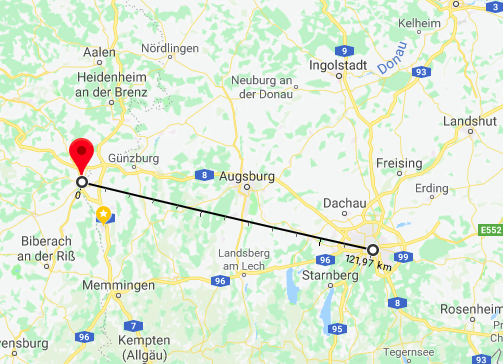
\includegraphics[width=0.8\textwidth]{img/fly}
\captionof{figure}{Compute Distances as the Crow Flies shown in Google Maps}\label{fig:fly}
\end{figure}
\subsubsection{Distances by Road}
There is not much library providing a routing algorithm for python and working with OpenStreeMap.
But we found \textbf{pyroutlib2} \citep{OpenStreetMap2017}. It does not seem to be supported therefore we
had to make a few modifications to the original code to make it work.\\
The modified version can be found in the NominatimLibrary GitHub repository.\\
The dependency osmapi is required.\\
First, we get the coordinates of the starting and finishing points:
\begin{lstlisting}[breaklines=true]
location = locator.geocode("Prittwitzstrasse, Ulm")
a = (location.latitude, location.longitude)
location = locator.geocode("Albert-Einstein-Allee, Ulm")
b = (location.latitude, location.longitude)
from pyroutelib2.loadOsm import LoadOsm
from pyroutelib2.route import Router
# By default, it uses the open API, this can be changed directly in the file
# Here, we use bicycle to calculate routes.
data = LoadOsm("cycle")
router = Router(data)
# This gets the node ids of the two points
node_a = data.findNode(a[0], a[1])
node_b = data.findNode(b[0], b[1])
# `doRoute` calculates the route and returns a list of coordinates tuples
result, route = router.doRoute(node_a, node_b)
if result == 'success':
# Do something...
pass
else:
print("Error calculating the route.")
\end{lstlisting}
Finally, to get the distance, we compute the distance between each couple of points:
\begin{lstlisting}[language=bash,breaklines=true]
from geopy import distance
lats = []
lons = []
if result == 'success':
for i in route:
node = data.rnodes[i]
lats.append(node[0])
lons.append(node[1])
else:
print("Error calculating the route.")
distance_route = 0
for i in range(len(lons)-1):
p1=(lats[i],lons[i])
p2=(lats[i+1],lons[i+1])
distance_route += distance.geodesic(p1,p2, ellipsoid='GRS-80').km
print("Total distance on the route : %.2fkm" % distance_route)
\end{lstlisting}
As a result we get from Prittwitzstrasse to Albert-Einstein-Allee, a distance by route of 5.87 km. 
Google Maps gives a similar result of 5.2 km as shown in figure \ref{fig:route}.
\begin{figure}[H]
\hspace{-1.3cm}
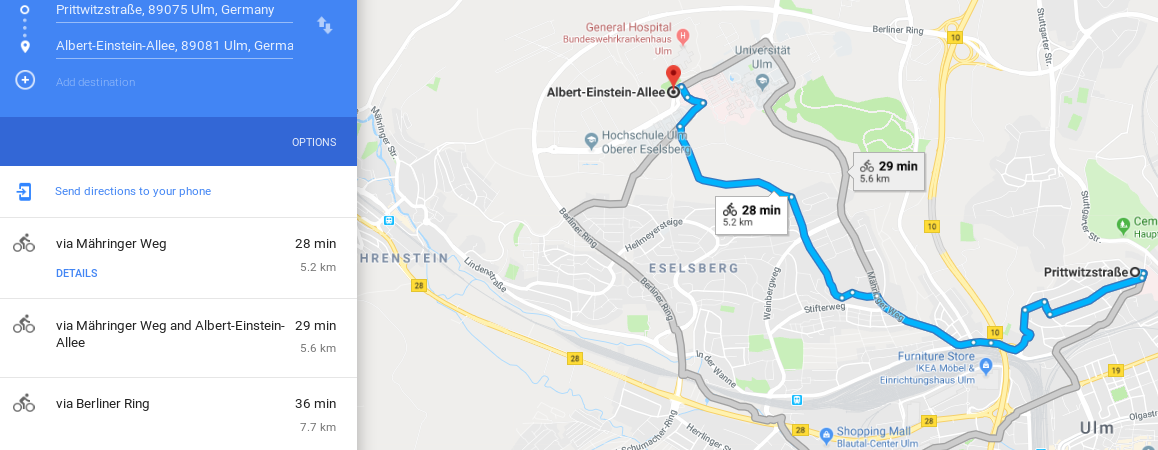
\includegraphics[width=1.3\textwidth]{img/route}
\captionof{figure}{Distance shown in Google Maps}\label{fig:route}
\end{figure}
\noindent For some in-city routes, the library is pretty fast, but for longer routes (Stuttgart $\rightarrow$ Muenchen), \textbf{pyroutelib2} took nearly an hour. Consequently, this is not a possible solution to calculate all the distances between postcodes. We will then have to turn to another way (external to python) of calculating the routes for the project.

% vim:ft=tex

\section{Graphhopper}\label{sec:graph}

Graphhopper is an open-source routing library and server written in Java which provides a web
interface called Graphhopper Maps as well as a routing API over HTTP.
\subsection{Deployment}
For simplicity you could just start jetty from maven and schedule it as background job: 
\begin{lstlisting}[language=bash,breaklines=true]
graphhopper.sh -a web -i europe_germany_berlin.pbf -d --port 11111
\end{lstlisting}
Then the service will be accessible on port 11111.
For production usage you have a web service included. Use \textbf{-c config.yml} in the script to point to
it. Increase the \textbf{-Xmx/-Xms} values of your server server e.g. for world wide coverage with a
hierarchical graph do the following before calling \textbf{graphhopper.sh}:
\begin{lstlisting}[language=bash,breaklines=true]
export JAVA_OPTS="-server -Xconcurrentio -Xmx17000m -Xms17000m"
\end{lstlisting}
Graphhopper is able to handle coverage for the whole OpenStreetMap road network. It needs
approximately 22GB RAM for the import (CAR only) and ~1 hour (plus ~5h for contraction). If
you can accept slower import times this can be reduced to 14GB RAM - you'll need to set
\textbf{datareader.dataaccess=MMAP}. Then 'only' 15GB are necessary. Without contraction hierarchy this would be about 9GB. With CH the service is able to handle about 180 queries per second (from localhost to localhost this was 300qps). Measured for CAR routing, real world requests, at least 100km long, on alinux machine with 8 cores and 32GB, java 1.7.0\_25, jetty 8.1.10 via the QueryTorture class (10
worker threads).\\
Especially for large heaps you should use \textbf{-XX:+UseG1GC}. Optionally add \textbf{-XX:MetaspaceSize=100M}.
Avoid swapping e.g. on linux via \textbf{vm.swappiness=0} in \textbf{/etc/sysctl.conf}.
If you want to use elevation data you need to increase the allowed number of open files. Under
linux this works as follows:
\begin{itemize}
\item sudo vi /etc/security/limits.conf
\item add: * - nofile 100000 which means set hard and soft limit of "number of open files" for all users to 100K
\item sudo vi /etc/sysctl.conf
\item add: fs.file-max = 90000
\item reboot now (or sudo sysctl -p; and re-login)
\item afterwards ulimit -Hn and ulimit -Sn should give you 100000
\end{itemize}
\subsection{Usage}
Our endpoint is \textbf{https://graphhopper.com/api/[version]/vrp}.
Graphopper can provide up to 6 APIs: 
\begin{itemize}
\item Routing API
\item Route Optimization API
\item Isochrone API
\item Map Matching API
\item Matrix API
\item ZGeocoding API
\end{itemize}
\subsubsection{Routing API}
Get distances between two points:
\begin{lstlisting}[language=bash,breaklines=true]
curl "https://graphhopper.com/api/1/route?
point=51.131,12.414&point=48.224,3.867&vehicle=car&locale=de&key=[YOUR_KEY]"
\end{lstlisting}
Example in our case:
\begin{lstlisting}[language=bash,breaklines=true]
https://localhost:11111/1/route
?point=51.131,12.414&point=48.224,3.867&vehicle=car&locale=de&key=3160e710-58ed-45da-
bb39-09d383b1c5b2
\end{lstlisting}
\subsubsection{Pricing}
The Graphhopper routing engine is open source under the permissive Apache License and is
therefore free to use for anything. You could even integrate it in your products, modify
Graphhopper and sell this, without noticing or contributing back. Although it is encouraged to
contribute back so that your feature gets maintained for free by graphhopper service. Also you
can host Graphhopper on your own servers for 'free' and do whatever you want with it.
The Graphhopper Directions API that we host falls under usage terms and always requires an
API key. It was decided to make it free for development purposes and open source projects,
both with a limit of currently 500 queries per day. So, the free usage of the API in a company
internally would not be allowed. But there are custom packages possible.\\\\
One Routing API request costs one credit. Every 10 via-points cost one more credit. E.g. 11 via-
points cost two credits, 21 via-points costs three credits and so on. And if you specify \textbf{optimize=true} the credits will be multiplied by 10 i.e. one requests costs 10 credits for 1 to 10 locations, 20 credits for 11 to 20 locations and so on. Changing the parameter algorithm costs additionally two credits, i.e. calculating the alternative route between two points costs 1+2=3 credits.
For more info about the other APIs:
\href{https://graphhopper.com/api/1/docs/FAQ/}{Graphhopper API Docs}

% vim:ft=tex

\section{Database}

Since we want to compute distances between the centroids of two postalcode areas we need a database where those information can be stored. 
\subsection{SQL vs NOSql}
First, it was necessary to find a suitable database. For this purpose we compared the \ac{nsql} and the \ac{sql} approaches with each other.\\
\acs{sql} happens to be the more structured, right way of storing data, like a phone book. For a relational database to be effective, you will have to store your data in a
very organized fashion. SQL databases remain popular because they fit naturally into many
vulnerable software stacks, including LAMP and Ruby-based stacks. These databases are widely
supported and well understood, which could be a major plus point if you run into problems.\\
The main problem with SQL is scaling it as your database grows. You see, even though
scalability is usually tested in production environments, it’s often lower than NoSQL
databases.\\\\
For dealing with massive amounts of unstructured data and data requirements which
aren’t clear at the outset, you probably don’t have the luxury of developing a relational database with
a clearly defined schema. You get much more flexibility than its traditional counterparts, with non-
relational databases. Picture non-relational databases as file folders, assembling related information
of all types.\\\\
Since we already know the scope of our database and therefore don`t want to scale it up and due to the lack of time and the good knowledge of team members in SQL, we decided to make use of the relational database \textbf{MySQL}.
\subsection{Installation}
Since MySQL is the most popular open-source relational database management system, we decided to install this system on our server. 
First we installed the MySQL package with the following command:
\begin{lstlisting}[language=bash,breaklines=true]
sudo apt install mysql-server
\end{lstlisting}
Once the installation is completed, the MySQL service will start automatically. To check whether the MySQL server is running or not, we type:
\begin{lstlisting}[language=bash,breaklines=true]
sudo systemctl status mysql
\end{lstlisting}
After we have made sure that the database is running, we create a user account:
\begin{lstlisting}[language=bash,breaklines=true]
CREATE USER IF NOT EXISTS 'database_user'@'localhost' IDENTIFIED BY 'user_password';
Copy
\end{lstlisting}
Afterwards a new database could be created and initialized.
\subsection{Datamodel}
To implement an appropriate database which offers fast responses to queries it was indispensable to design a datamodel which fulfills these requirements. The figure \ref{pic:er} shows the output of the datamodelling process.
\begin{figure}[H]
\hspace{1.2cm}
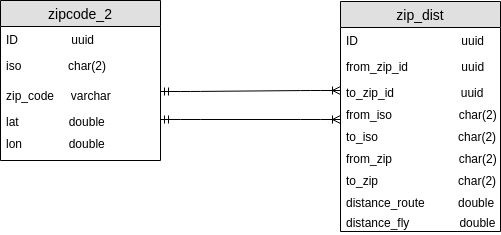
\includegraphics[width=0.8\textwidth]{img/er}
\captionof{figure}{ER model for the MySQL Database}\label{pic:er}
\end{figure}
\noindent The model consists of two entities which are connected over a one-to-many relationship.
The datamodels for the postcodes and the distances were directly written in the Django source code. That way, Django directly provides a python object to work with the tables. It is even possible to write methods to manipulate this data directly from it. The implementation is done in the file:
\href{https://github.com/dataBikeHsUlm/WebApp/blob/master/geonom/datamodel/models.py}{model.py}.
For further information on working with the database in Django, see our corresponding 
\href{https://github.com/dataBikeHsUlm/WebApp/blob/master/django_recap.md#database}{GitHub repository}.
\subsection{Initialize Database}

\subsubsection{Geonames}
To be able to fill the postalcode table, we need a list of all postcodes per country. The Nominatim API doesn't directly provide a function to do that, however the \emph{GeoNames}, which is a geographical database, provides a list of all postalcodes which are free to download \citep{GeoNames}.
We implemented a first version of a script using this list and started filling the database.
Geonames was incomplete, some countries (like Greece) were missing and the script had problems finding some cites.  Therefore we had to find another, more reliable way to get the postcodes.

\subsubsection{Nominatim Database}
We decided to directly look into the Nominatim PostgreSQL database. There is in fact a table named
\textbf{location\_area} containing the column postcodes and the related \textbf{country\_code} .
Some rows in this table have empty \textbf{country\_code} or \textbf{postcode}, so we need to filter them out. The resulting SQL query looks as followed:
\begin{figure}[H]
\hspace{1.2cm}
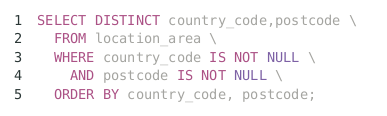
\includegraphics[width=0.55\textwidth]{img/query1}\label{pic:q1}
\end{figure}
Then, for every postcode, we need to query the Nominatim API to get the centroid
coordinates, but querying only with the country code and the postcode is too ambiguous
and can lead to wrong centroids.
To fix that, we used the \textbf{country\_name} table that lists countries with
names and ISO codes. We joined this table to the previous one:
\begin{figure}[H]
\hspace{1.2cm}
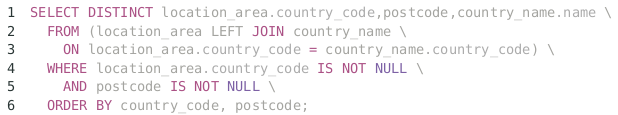
\includegraphics[width=0.9\textwidth]{img/query2}\label{pic:q2}
\end{figure}

\subsubsection{Final Script}

To ensure that we don't left out any postal codes, we use both sources to fill
the database.
In the table, 443493 postcodes from 51 countries were inserted with this script.
Using the resulting data, the script to fill the zipcode table was re-written, the database cleaned and filled with the new version of the script. The script can be found at the GitHub repository \href{https://github.com/dataBikeHsUlm/WebApp/blob/master/fill_db_postcodes.py}{WebApp}.
To run the script, run the accompanying shell script \textbf{fill\_db.py}, it will install the dependencies before running the python code.

% vim:ft=tex

\section{Distance Database}

\subsection{Algorithm}

If we computed the distance between all cities in Europe, it would take a very
long time and file the hard drive consequently.
To reduce the effort was decided to group each postcode by its region (most of the
time represented by the two first digits). Then we compute the distance ``as the
crow flies'' and by road between each of these regions and store them into the database.

When requesting the distance between two postcode, we process as such:
\begin{enumerate}
  \item transform both postcode into coordinates
  \item calculate the distance as the crow flies (named $d_{direct,crow}$)
  \item determine the two 2-digit regions associated
  \item get the distance ``as the crow flies'' ($d_{region,crow}$) and by road
      ($d_{region,road}$) between the two regions from the database
  \item calculate the ratio $ratio = d_{region,road}/d_{region,crow}$
  \item the final distance estimate is $d_{direct,crow} * ratio$
\end{enumerate}

The calculation is summarized by figure~\ref{fig:calc}.
\begin{figure}[H]
\centering
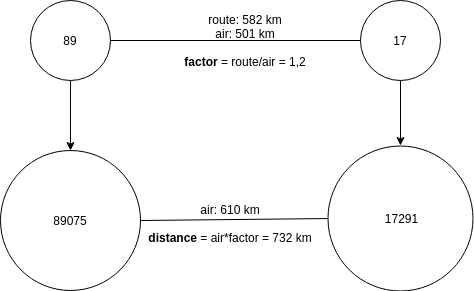
\includegraphics[width=0.7\textwidth]{img/calc}
\captionof{figure}{Theoretical example of distance calculation}\label{fig:calc}
\end{figure}

\subsection{2-digits Database}

\subsubsection{List of 2-digits Regions}

The countries' regions being often indicated as the two first digits of the
postcodes, we can simply create our groups based on that.
However, we must take into account that there are some exceptions; for instance,
Luxembourg prefixes its postcodes with ``LE-''.
Some other countries also introduce non-alphanumerical characters, such as:
spaces, hyphens, dots, \ldots{}

We also restrict this operation to European countries only, we can do that by filtering
postcodes by their coordinates: Europe being found between -11° West and 41° East,
and 35° to 71° North.

\subsubsection{Calculation of a Region's Centroid}

To calculate the centroid for each region, we can compute the average coordinates
of all postcodes of that region. However, we will have to use Graphhopper with
these coordinates and Graphhopper can only work when coordinates point to a
road/street/\ldots{}
To test if a coordinate is working for Graphhopper, we simply query it from our
coordinate to an already checked place.

First, we test Graphhopper for the average centroid. If it can't be used, we go
through the closest postalcodes to find one accepted by Graphhopper. Finally, if
we still don't have a good point, we spiral around the average centroid until we
find a good point or we reach 3 degrees radius (3 degrees in longitude is around
245km in Germany). We discard every other regions that fail these three tests.

\subsubsection{Filling the Database}

For each couple of region centroids calculated above, we calculate the distance
``as the crow flies'' thanks to the GeoPy function and the distance by road thanks
to Graphhopper API and store those two results in the MySQL database.

The script can be found at the GitHub repository \href{https://github.com/dataBikeHsUlm/WebApp/blob/master/fill_db_with_distances_2digits.py}{WebApp}.

% vim:ft=tex

\section{Django Web Application}\label{sec:django}

% Since we only have a limited amount of time working on the project we decided to do expert based learning on Django. This means only one of us will research for the usage and implementation of Django to subsequently teach his findings to the team.
% Therefore Guillaume Goni wrote a recapitulative document for the rest of the team, so everyone could quickly get ready to work on the server code.
% It is mostly inspired by the official tutorial of Django \citep{Djangodocumentation2019} and from the Django documentation \citep{Django2019}.\\
% Due to the lack of time it wasn't`t already possible to implement the WebApp using the Django framework. This will be part of the next sprint.
% As already mentioned in chapter~\ref{sec:django} we already researched for the Django framework in the past semester, however the implementation of the Django web application was rescheduled to this part of the masterproject.

The aim of this task was to develop a web application to provide distance calculation based on our Nominatim as well as our Graphhopper server. The calculation should be done by postalcodes as well as iso codes. As a result it should return the air distance as well as the distance by route of the related postalcodes.

\subsection{Mockup}

After the requirements were clear, we designed a mockup (see figure~\ref{fig:mockup}) in order to define the layout of the web application.

\begin{figure}[H]
\centering
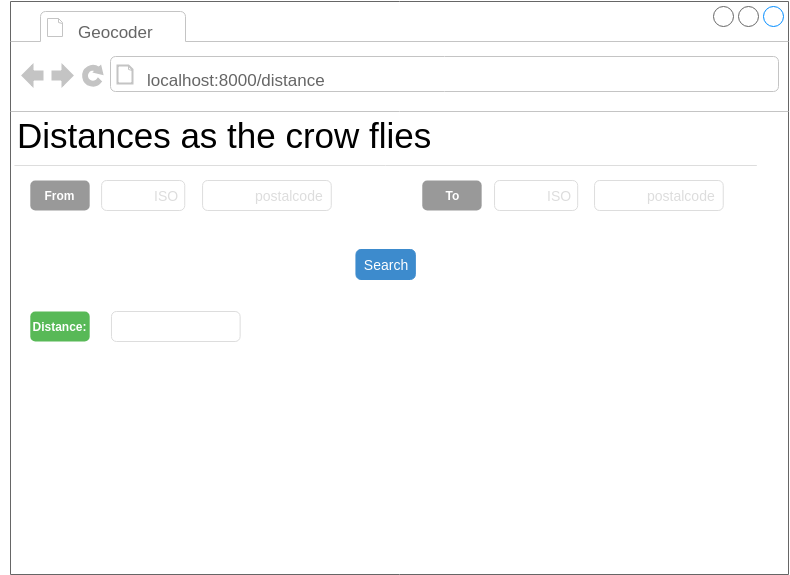
\includegraphics[width=0.8\textwidth]{img/mockup}
\captionof{figure}{Mockup for Django web app}\label{fig:mockup}
\end{figure}

The mockups shows four input fields where the user can enter the postalcode and the corresponding iso code of his start and his starting point as well as his destination. The \glqq Search\grqq-button triggers the calculation and represents the result in the input field with the label \glqq Distance\grqq below. In this mockup only the distance calculation as the crow flies was taken into consideration. However in the final web application we included the distance calculation by route as well.\\

\subsection{Implementation}

For our frontend web application, we will use \textbf{Django} as it works in python and is the most used.

\subsubsection{View}

This mockup was then implemented as an HTML file. In order to get a quick result with a sophisticated and responsive design we decided to include the Bootstrap toolkit. This open source framework provides themes, templates and code snippets for a uniform layout and rapid processing. Therefore we installed bootstrap on our Nominatim server.
The view consist mainly of four parts:
\begin{enumerate}
\item index.html
\item style.css
\item urls.py
\item views.py
\item forms.py
\end{enumerate}
The \emph{index.html} file is responsible for the general structure of the web application. The \emph{style.css} file is mainly responsible for the layout of the footer which is customized and not just adapted by bootstrap. \\
In the \emph{urls.py} we defined which HTML file should be displayed for which url. Since the web application consist of one page only we set the index.html as the entry point by calling the web application. \\
Django provides a very secure form handling which is normally a very complex business including editing the form with a convenient interface, send it to the server, validate and clean the input and then save or pass it to further processing. With Django's form functionality all this work is automated and also do it more securely then we would probably be able to do.
Therefore we created the file \emph{forms.py} where we directly specified the input fields with their corresponding length as well as if they are required or not.
\begin{lstlisting}[language=python,breaklines=true]
class CrowForm(forms.Form):
    from_zip = forms.CharField(max_length=5,required=True)
    from_iso = forms.CharField(max_length=2,required=True)
    to_zip = forms.CharField(max_length=5,required=True)
    to_iso = forms.CharField(max_length=2,required=True)
    \end{lstlisting}
The input of this form is then processed within the \emph{views.py} file, since here the post and get requests are handled.
The \emph{views.py} file is responsible to handle post ad get requests.
This file calls also the responsible methods of the datamodel in order to calculate the distances.
Moreover it returns the results to the input fields \glqq Direct\grqq and \glqq By route\grqq which can be seen in figure~\ref{fig:webapp}.
\begin{figure}[H]
\hspace{-2.0cm}
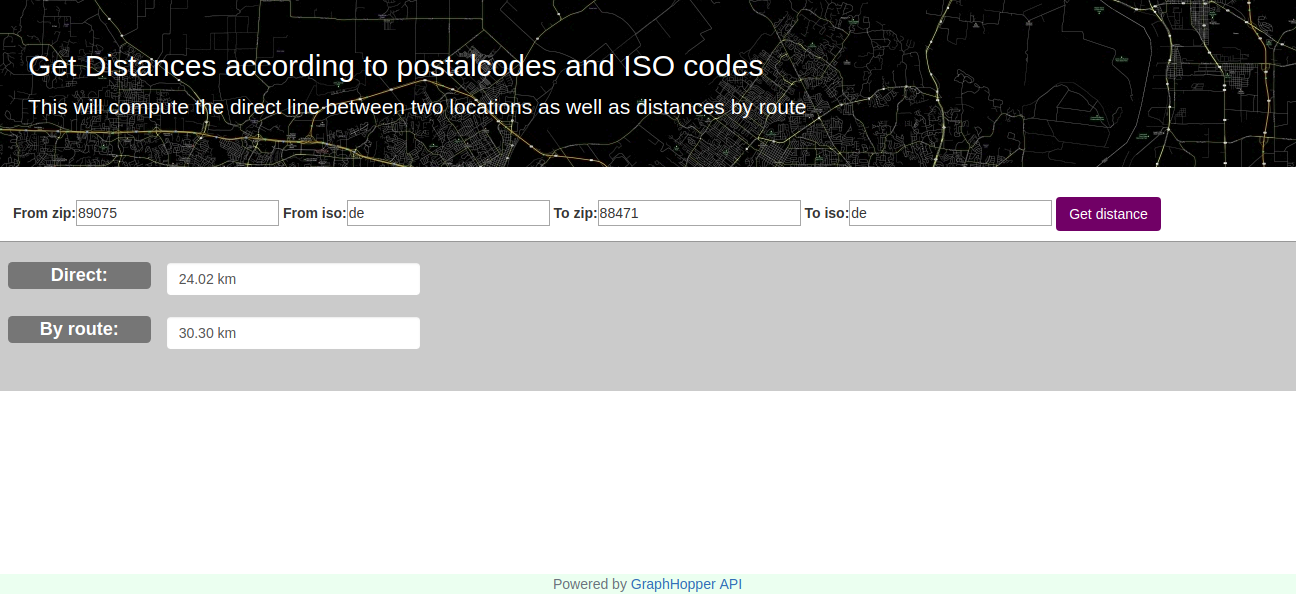
\includegraphics[width=1.3\textwidth]{img/webapp}
\captionof{figure}{Final layout of the Django web application}\label{fig:webapp}
\end{figure}

%%%%%%%%%%%%%%%%%%%%%%%%%%%%%%%%%%%%%%%%%%%%%%%%%%%%%%%%%%%%%%%%%%%%%%%%%%%%%%%%%%%%%%%%%%%%%%
%%%%%%%%%Have fun Guillaume no it is your turn:-)%%%%%%%%%%%%%%%%%%%%%%%%%%%%%%%%%%%%%%%%%%%%%
\subsubsection{Calculation}

%%%%%%%%%%%%%%%%%%%%%%%%%%%%%%%%%%%%%%%%%%%%%%%%%%%%%%%%%%%%%%%%%%%%%%%%%%%%%%%%%%%%%%%%%%%%%%
%please add here the calculation bla bla bla

\chapter{Bike Rental in London}
% vim:ft=tex

\section{Evaluation of Hadoop Distributions}

This chapter shows a general conducted comparison of Hadoop distributions which are dominating the big
data market. Since it is necessary for our data science project to compute in a parallel and efficient fashion, such a comparison helps us to identify the right distribution. Firstly, an overview of the identified distributions with its features and pricing tiers will be showed. Afterwards we will declare some important criteria for our project based on an extensive research of internet blogs and manufacturer websites. Then a weighting of these criteria will be done. These criteria will be used to evaluate the different Hadoop distributions. The resulting evaluation matrix shows that Hortonworks might be the best distribution for our data science problem. However, a detailed look at the performance criterion shows us that MapR is the most most powerful in five5 out of six cases. For this performance comparison, evaluation results of various MapReduce jobs found on the Internet are used. Hence, in a pure performance comparison MapR would win over Hortonworks, but in an overall comparison Hortonworks convinces more. To round off the
evaluation, a test implementation of Hortonworks was carried out on the four virtual machines procured for
this purpose where some simple MapReduce jobs are carried out.
\subsection{Hadoop Distributions Overview}\label{hd}
For the first part of the evaluation, a search for widespread Hadoop distributions was conducted \citep{hadoopvendors,forrester,comparison2014,Cloudera,M.Heo2015}.
As the table~\ref{tab:distributions} below shows, seven noteworthy distributions were found.
%\hspace{-2.5cm}
\begin{table}[H]
%\centering
\hspace{-3.3cm}
\begin{tabular}{|p{4.4cm}|p{6.2cm}|p{4cm}|p{4cm}|}
	\hline
	\textbf{Hadoop \newline Distribution} & \textbf{Features} & \textbf{ Pricing Gear}  & \textbf{ Hadoop \newline Ecosystem}\\ \hline
	Apache Hadoop 3.1.1
\href{http://hadoop.apache.org/}{hadoop.apache.org} & 
\begin{itemize}[noitemsep,leftmargin=*]
   \item No extra tools
   \item Blank installation of Apache Hadoop (HDFS, YARN and Hadoop Web UI)
\end{itemize}
& Open Source 100\% & Has to be
installed
manually \citep{apachehadoop}\\ \hline
Cloudera CDH (v5.15.0)
\href{https://www.cloudera.com/}{www.cloudera.com} & \begin{itemize}[noitemsep,leftmargin=*]
   \item Oldest distribution
   \item Very polished
   \item Comes with good (and proprietary)
tools to install and manage a Hadoop
cluster: \begin{itemize}
\item Cloudera Manager for managing
and monitoring clusters \citep{Cloudera2018a}.
\item Cloudera Search (Free-Text) on
Hadoop \citep{Cloudera2018}.
\item Apache Crunch framework for
MapReduce Pipelines \citep{Cloudera2018}.
\end{itemize}
\end{itemize} &Freemium (Cloudera Manager require license). Also source code is not fully available and enterprise edition has 60 trial-day \citep{D.Kumar2016}. Final costs may depend on cluster size \citep{Cloudera}.  &Accumulo,Flume, HBase, HCatalog, Hive, HttpFS, HUE, Impala, Kafka, KMS, Mahout, Oozie, Pig, Sentry, Snappy, Spark, Sqoop, Parquet, Whirr, ZooKeeper \citep{Cloudera2018a,Cloudera2018}\\ \hline
\end{tabular}
%\caption{Vergleich ausgewählter Column Family Datenbanken (eigene Darstellung)}
\label{tab:distributions}
\end{table}
%end first table!
\vspace{-2.5cm}
\begin{table}[H]
%\centering
\hspace{-3.3cm}
\begin{tabular}{|p{4.4cm}|p{6.2cm}|p{4cm}|p{4cm}|}
	\hline
	\textbf{Hadoop \newline Distribution} & \textbf{Features} & \textbf{ Pricing Gear}  & \textbf{ Hadoop \newline Ecosystem}\\ \hline
Hortonworks Data
Platform (HDP3.0.1)
\href{https://hortonworks.com/}{www.hortonworks.com} &\begin{itemize}[noitemsep,leftmargin=*] \item Newer distributions
\item Tracks Apache Hadoop closely
\item Comes with standard and open source
tools for managing clusters:
\begin{itemize}
\item Improved HDFS in HDP 2.0:
automated fail over with a hot
standby and full stack resiliency
\citep{Hortonworks2018c}.
\item Ambari for managing and monitoring clusters. \item Includes almost all Hadoop
extensions from the Apache
foundation \citep{Hortonworks2018c}.
\end{itemize}
\end{itemize} & Open Source, optional enterprise paid support \citep{D.Kumar2016} &Atlas, HBase, HDFS, Hive Metastore, HiveServer2, Hue, Spark, Kafka, Knox, Oozie, Ranger, Storm, WebHCat, YARN, SmartSense, ZooKeeper \citep{Hortonworks2018b} \\ \hline
MapR 6.1 \href{https://mapr.com/} {www.mapr.com} &\begin{itemize}[noitemsep,leftmargin=*] 
\item Uses own HDFS (MapR-FS)
\item Integrates own database systems (MapR-DB seven times faster than HBase)
\item Mostly used for big big data projects
\item Free from Single Point of Failures
\item Offers Mirroring and Snapshotting
\item Might be the fastest Hadoop distribution 
\item MapR supports backward compatibility across multiple version of projects
\item Supports a global event replication for streaming at IoT scale (MapR-ES)
\end{itemize}& Freemium \citep{MapR2018b}:Community Edition contains no high availability, no disaster recovery and no global replication for streaming data.& AsyncHBase, Cascading, Drill, Flume, HBase Client and MapR Database, Binary Tables, Spark, HCatalog, Hive, HttpFS, Hue, Impala MapR Event Store For Apache Kafka Clients and Tools, Myriad, OpenStack, Manila, Oozie, Pig, Sentry, Spark, Sqoop, MapR Object Store with S3- Compatible API\citep{MapR2018a}\\ \hline
\end{tabular}
\label{tab:distributions}
\end{table}
%end second table!
\begin{table}[H]
\hspace{-3.3cm}
\begin{tabular}{|p{4.4cm}|p{6.2cm}|p{4cm}|p{4cm}|}
	\hline
	\textbf{Hadoop \newline Distribution} & \textbf{Features} & \textbf{ Pricing Gear}  & \textbf{ Hadoop \newline Ecosystem}\\ \hline
Intel
\href{https://http://hadoop.intel.com/}{www.hadoop.intel.com}
&\begin{itemize}[noitemsep,leftmargin=*] 
\item Partnered with Cloudera \citep{MervAdrian2017}
\item Encryption support
\item Hardware acceleration added to layers of stack to boost performance
\item Admin tools to deploy and manage Hadoop
\end{itemize}&
Premium (90 days trial) & Offers same
services as
Cloudera. \\ \hline
Pivotal HD
 \href{https://gopivotal.com//} {www.gopivotal.com} &\begin{itemize}[noitemsep,leftmargin=*] 
\item Partnered with Hortonworks \citep{MervAdrian2017}
\item Fast SQL on Hadoop
\item Proprietary Software \citep{Pivotal2018}:
\begin{itemize}
\item Pivotal DataLoader
\item USS (external file system)
\item Spring Data
\item Pivotal ADS-HAWQ (parallel SQL query engine)
\end{itemize}
\end{itemize}& Premium &Offers same services as Hortonworks.\\ \hline
IBM Open Platform
\href{https://www.ibm.com/de-de/?ar=1}{www.ibm.com}&\begin{itemize}[noitemsep,leftmargin=*] 
\item Partnered with Hortonworks \citep{MervAdrian2017}
\item Proprietary tools:
\begin{itemize}
\item IBM Big SQL allows concurrent process of Hive, HBase and Spark and other sources using a single database connection \citep{MervAdrian2017}.
\item IBM BigInsights v4.2 provides Text-Analytics module \citep{I.K.Center2018}.
\end{itemize}
\item Highly compatible to other IB products.
\end{itemize}
&Free for non-commercial purposes, optional enterprise paid support \citep{IBMAnalytics2018}
& Offers same services as Hortonworks.\\ \hline
\end{tabular}
\caption{Overview of Hadoop distributions}
\label{tab:distributions}
\end{table}
\noindent It is worth to mention that each Hadoop distribution in table \ref{tab:distributions} comes up with a minimum of services from the Apache foundation: \ac{yarn}, \ac{hdfs}, Hive, Pig, HBase, Kafka, Storm, Mahout, HCatalog... But they may use a proprietary implementation of them e.g. MapR uses own HDFS instead of Apache HDFS implementation. It is also worth to note that a few cloud providers are offering Hadoop cluster services over their platforms. For instance, Microsoft Azure provides with HDInsight a full manageable Hadoop respectively Spark Cluster \citep{Microsoft2018}. The user could profit from fast provisioning and also from less costs since no on-prem hardware cluster infrastructure is required. Therefore, Hadoop (or better Spark) by Cloud Computing is also a noteworthy option for our data science project in the future, although it may be over sized at the moment. It is worth to mention that each Hadoop distribution in table \ref{tab:distributions} comes up with a minimum of services from the Apache foundation: YARN, HDFS, Hive, Pig, HBase, Kafka, Storm, Mahout, HCatalog etc. But they may use
a proprietary implementation of them e.g. MapR uses own HDFS instead of Apache HDFS implementation. 
It is also worth to note that a few cloud providers are offering Hadoop cluster services over their platforms. 
For instance, Microsoft Azure provides with HDInsight a full manageable Hadoop respectively Spark Cluster
\citep{Microsoft2018}. The user could profit from fast provisioning and also from less costs since no on-prem hardware
cluster infrastructure is required. Therefore, Hadoop (or better Spark) by Cloud Computing is also a
noteworthy option for our data science project in the future, although it may be over sized at the moment.\\\\
Nevertheless, Intel, ERM/Pivotal and IBM partnered with Hortonworks or Cloudera \ref{tab:distributions}. These vendors therefore have the same extensions as their partners offer, but also can provide exclusive tools for users (e.g. IBM Big SQL \citep{MervAdrian2017}). If we take this into account, we find that there are mainly 3 different Hadoop distributions: Cloudera with CDH, Hortonworks with its \ac{hdp} and MapR with its own HDFS. In addition to the distributions shown in \ref{tab:distributions}, there are many other Hadoop distributions such as Altiscale from SAP or Elastic MapReduce from Amazon. Both run only in a cloud environment. The Forrester Wave shows also the three global players Cloudera, Hortonworks and MapR (see \ref{pic:forrester}). Since cloud solutions do not play a role for this use case, Microsoft, Google or Amazon will not be considered.
\begin{center}
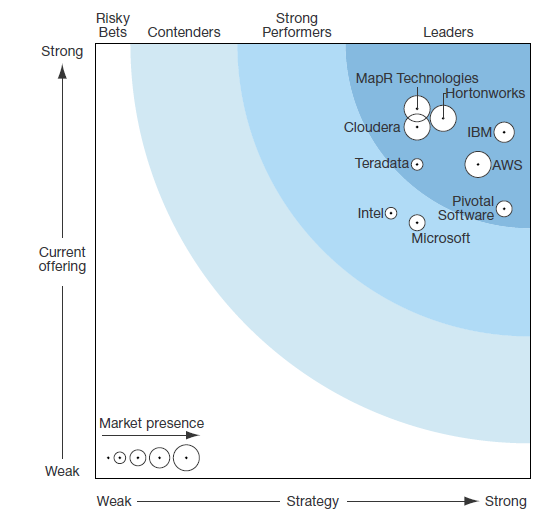
\includegraphics[width=0.8\textwidth]{img/figure1}
\captionof{figure}{Forrester Wave of Hadoop Distributions \citep{forrester}}\label{pic:forrester}
\end{center}
As we can see from 
\ref{pic:forrester} 
the three mentioned Hadoop distributions are building a cluster and Cloudera
even overlaps with MapR slightly. That means, they are providing similar products and enjoy a similar
market position. From the Forrester Wave (\ref{pic:forrester}) we can derive that MapR seems to have the best offering. However, since we want to use one of them for our analytics project we have to dig a step deeper and make a decision based on well-defined criteria.
\subsection{Definition of criteria}
Hadoop distributions are rated using selected criteria, with scores ranging from 1 (very poor) to 5 (very
good). Based on the research carried out, the following 20 clear criteria can be determined:
\begin{table}[H]
\hspace{-1.6cm}
\begin{tabular}{|l|l|}
\hline
\textbf{Criterion}             & \textbf{Description}                                                                                                                                                     \\ \hline
Batch Processing               & \begin{tabular}[c]{@{}l@{}}Batch process jobs can run without any end-user\\ interaction or can be scheduled to start up on their own\\ as resources permit\end{tabular} \\ \hline
Cloud Support                  & Cloud compatibility of Hadoop distributions                                                                                                                              \\ \hline
Cluster Scalability            & \begin{tabular}[c]{@{}l@{}}Creating new clusters ad-hoc and set up cluster size\\ (e.g. 4,8 or 12 nodes)\end{tabular}                                                    \\ \hline
Data querying possibilities    & \begin{tabular}[c]{@{}l@{}}Ways to query Hadoop with SQL (e.g. Hive, Stinger,\\ Spark SQL,...)\end{tabular}                                                              \\ \hline
Database Support               & \begin{tabular}[c]{@{}l@{}}Additional databases in Hadoop (e.g. PostgreSQL,\\ MongoDB, HBase, Impala etc.)\end{tabular}                                                    \\ \hline
Disaster-Discovery             & \begin{tabular}[c]{@{}l@{}}There is a fallback option available in case of\\ unexpected Hadoop errors\end{tabular}                                                       \\ \hline
Ease of Use                    & The complexity of the usage of the Hadoop distribution                                                                                                                   \\ \hline
High-Availability               & \begin{tabular}[c]{@{}l@{}}Self-healing across multiple services or single failure\\ recovery (i.e. fail-over clusters)\end{tabular}                                     \\ \hline
Install complexity             & \begin{tabular}[c]{@{}l@{}}Is there a simple installation routine or does it require\\ lot of manual configuration (e.g. Multi node Cluster...)?\end{tabular}             \\ \hline
Licensing and Pricing          & Cost model of Hadoop distributions                                                                                                                                       \\ \hline
ML support                     & \begin{tabular}[c]{@{}l@{}}Providing interface for enlarged machine learning tasks\\ (e.g. Spark MLlib...)\end{tabular}                                                  \\ \hline
Operating System Support       & Guaranteed and certified OS compatibility                                                                                                                                \\ \hline
Performance                    & \begin{tabular}[c]{@{}l@{}}Cluster performance in case of parallelized MapReduce\\ Jobs\end{tabular}                                                                     \\ \hline
Programming Language Support   & \begin{tabular}[c]{@{}l@{}}Support of data science programming languages\\ (Python and R)\end{tabular}                                                                   \\ \hline
Streaming Analytics            & \begin{tabular}[c]{@{}l@{}}Vendor offering real-time analytics capabilities (e.g. IoT\\ platform hub..)\end{tabular}                                                     \\ \hline
Support of secondary services  & Services on top of Hadoop (e.g. Zookeeper, Spark...)                                                                                                                     \\ \hline
Third party module integration & Usage of additional components from other vendors                                                                                                                        \\ \hline
User Support/Community         & How fast is the response in the community?                                                                                                                               \\ \hline
Expertise                      & Experience with Hadoop (life time of company, ...)                                                                                                                       \\ \hline
\end{tabular}
\caption{Definition of criteria}
\label{tab:criteria}
\end{table}
\noindent The weight scale ranges from 1 (trivial) to 4 (very important), with the focus on our Santander Bicycle project. This means that cloud support, for example, is a crucial criterion in many use cases, but has only little importance for our project which leads to a trivial weight. A percentage weighting is not applied because 20 criteria would result in a fine-granular distribution (which is not good to read at all). Therefore, absolute values are used for the comparison \ref{pic:matrix} in the next section.
\subsection{Weighted evaluation matrix}\label{weight}
As already mentioned in Section \ref{hd}, the three major Hadoop distributions are: Cloudera CDH 5.15.0,
Hortonworks HDP 3.0.1 and MapR 6.1.0. With regard to the defined comparison criteria, a weighted
decision matrix can be mapped. At the same time, this matrix represents the starting point for the decision of a Hadoop distribution. It cannot be denied that a certain degree of subjectivity is included in the evaluation (table \ref{tab:criteria}). In addition, only free editions are compared. For example, if a feature only exists in the premium version, this feature will be rated one (worst) since we don’t want to spend money.
\begin{center}
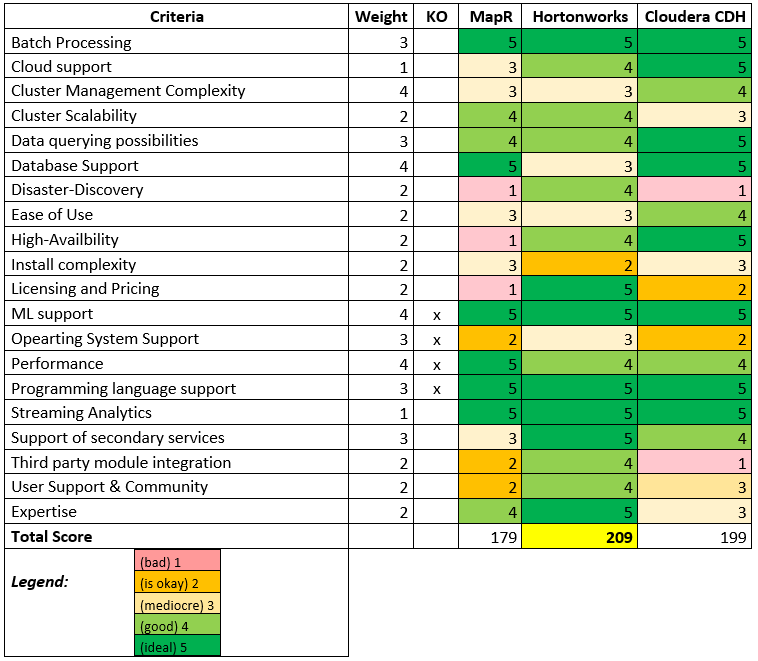
\includegraphics[width=1.0\textwidth]{img/matrix}
\captionof{figure}{Weighted Comparison Table of Hadoop Distributions}\label{pic:matrix}
\end{center}
The comparison in figure \ref{pic:matrix} clearly shows that there are almost no significant differences between the selected distributions. Although there are a few deviations such as disaster-discovery or pricing model, the overall distribution of points is relatively the same. From the comparison matrix it can be deduced that Hortonworks HDP achieves the highest score and is probably the best option for our project at the moment. It is possible that after the first test phase (see chapter \ref{intallhadoop}), it turns out that the distribution is not convenient after all which may require to update the evaluation matrix. Therefore figure \ref{pic:matrix} can be considered as a continuous iterative updateable weighted comparison matrix that will likely be updated on further sprints. Another representation of the evaluated Hadoop distributions, a spider chart may be appropriate as it makes it easier to read and to identify outliers or similarities even quicker as with a raw table.
\begin{center}
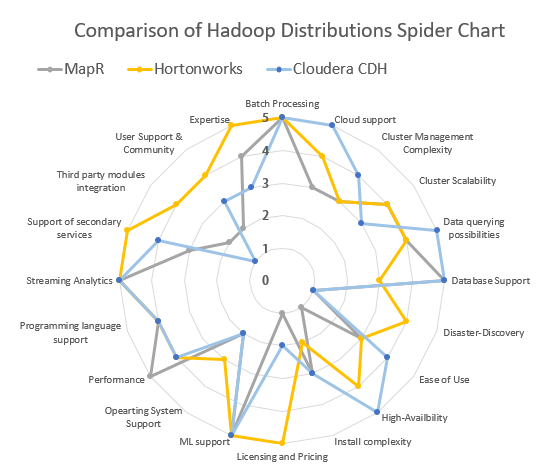
\includegraphics[width=1.0\textwidth]{img/spider}
\captionof{figure}{Spider Chart of compared Hadoop Distributions}\label{pic:spider}
\end{center}
The KO-criteria from figure \ref{pic:matrix} are all satisfied by the selected Hadoop vendors. One criterion that stands out is the license model, which was rated with 1 point for MapR and 2 points for Cloudera. This is due to the fact that the price models of both vendors are not transparent. So Cloudera offers a free community edition but to use the Cloudera Manager (the real strength of Cloudera) you have to pay again. Only Hortonworks offers a complete Open Source package with except the Hortonworks business support is fee required. However, Hortonworks has a very active community as well. MapR comes off worst with the criterion “Support of secondary services”, because there is no Spark and
HBase support in the "Converged Community Edition" \citep{MapR2018b}, but both are important Hadoop components for our project. So if we wanted to use MapR, we would have to use the paid version. There are also some other differences in figure \ref{pic:spider} such as Disaster-Recovery which is only on Hortonworks’s HDP completely free. An interesting aspect of the comparison is the performance criterion where MapR has the most points. Since this criterion is a KO-criterion that means it is a very important component for our project, it makes sense to examine the performance comparison between the distributions in a more detailed fashion.
\subsection{Performance Comparison with micro benchmarks}
For a performance comparison it is good to know how fast they compute when running in a
concurrent mode. For this task MapReduce Jobs like WordCount or \ac{dfsio} Read/Write might be helpful. Following figures are extracted from a sophisticated evaluation work by Altoros \citep{altoros}.
\begin{center}
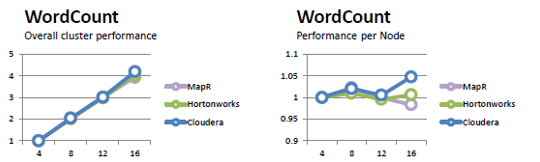
\includegraphics[width=1.0\textwidth]{img/bench1}
\vspace{0.1cm}
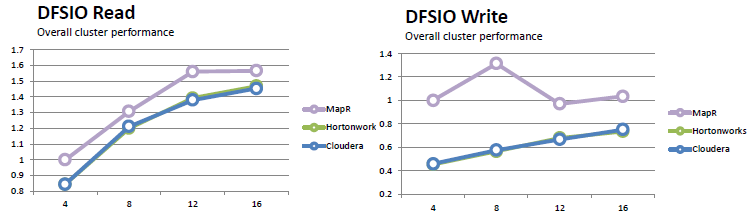
\includegraphics[width=1.0\textwidth]{img/bench2}
\captionof{figure}{Micro benchmarks on DFSIO / WordCount MapReduce Jobs}\label{pic:benchmarks}
\end{center}
For the performance comparison of figure \ref{pic:benchmarks} Hadoop cluster each one with 16 nodes have been established in order to measure computation time. An interesting point is that all three Hadoop distributions almost achieve the same overall speed on the famous WordCount MapReduce job. But if we look at the performance per node then there is a small difference between them. This could be due to a certain error rate in the execution of the job. If the same test were repeated, the results would be negligibly different. The DFSIORead/Write (figure \ref{pic:benchmarks}) job shows MapR is definitely faster than Hortonworks and Cloudera. The reason for
this might be the fact that MapR uses its own HDFS which is according to the vendor seven times faster
than the original one from Apache. This is the reason why it gets five points in the evaluation matrix (see table \ref{tab:criteria}) whereas other ones only reach four points. Hortonworks and Cloudera seems to have the same performance on the DFSIO job because both using Apache HDFS.\\In overall, Hortonworks HDP wins the competition for the moment, because they have the longest experience and are completely compatible with secondary services. Based on the evaluation matrix from chapter \ref{weight} and the performance measurements, it can be deduced that MapR is the most powerful Hadoop distribution on the market today, but when considering the other criteria, Hortonwork's Hadoop is simply more convincing. Especially the complete Open Source guarantee at Hortonworks is a decisive criterion for the choice of this distribution.\\Beside from the comparison, we would generally recommend to use rather Spark than Hadoop since Spark is around 100 times faster due to in-memory processing. Also Spark provides the most important libraries (ML, Streaming, etc) for data science and works well on top of Hadoop (thanks YARN). It can even be installed in a standalone manner, even though it doesn’t benefit from distributive multi mode computing.
\subsection{Installation of sample Hadoop Distribution}\label{intallhadoop}
Hortonworks offers a configurator on their website that can be used to check products, operating systems,
databases, browsers, JDKs and supported processors. It is noticeable that Ubuntu is only supported up to
16.04 LTS. However, our VMs are already v.18.4 LTS. This means Hortonworks does not official support
our installed OS \citep{Hortonworks2018a}. Also Cloudera CDH 5.15 \citep{Cloudera2018b} and the newest MapR 6.1 distribution \cite{MapR2018} only support Ubuntu 16.04 LTS (Xenial). Anyway, it is still a worth a try to set up \acs{hdp} Cluster on our virtual machines since the vendors are not explicitly warning Ubuntu 18.04 is not supported. So it may work. For the installation of HDP 3.0.1 the Ambari Wizard \citep{Hortonworks2018} will be used.\\First of all, we have to configure the \textbf{etc/hosts} since every node in the cluster must be able to communicate with each other. The hosts file should look like this:
\begin{figure}[H]
\hspace{-1.3cm}
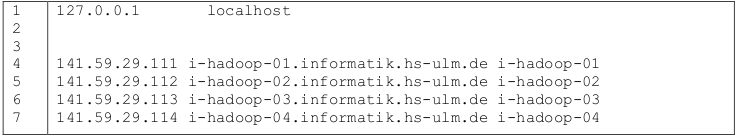
\includegraphics[width=1.2\textwidth]{img/etchost}
\captionof{figure}{etc/hosts configuration file}\label{pic:etchost}
\end{figure}
\noindent After that step, it is necessary to add public key authentication with SSH. The master node (\textbf{i-hadoop-01}) should login to its worker nodes without using a password. We can achieve this goal by generating a private / public key pair and distribute the public key to the 3 worker nodes by using \textbf{ssh-copy-id} command. Also for using Ambari the Hadoop user need sudo execution without password. Adding an additional line to \textbf{visudo} configuration file should solve that issue. At next, all nodes need to have Java installed. Since Ubuntu 18.04 doesn’t come up with a default Java JDK
we install Oracle JDK 1.8 manually on each node. After that it is time to download the Ambari repository
file to a directory on our Hadoop master host. The Ambari v. 2.7.1.0 is used for installation. With the command \textbf{apt-get install ambari server} the server will be installed on i-hadoop-01. Afterwards, we can start the server. Now we can go to the Ambari surface via following link: \href{http://i-hadoop-01.informatik.hs-ulm.de:8080}{http://i-hadoop-01.informatik.hs-ulm.de:8080}. The default login credentials are \textbf{admin admin}. After successful login, the real installation process begins.
\begin{figure}[H]
\hspace{-2.3cm}
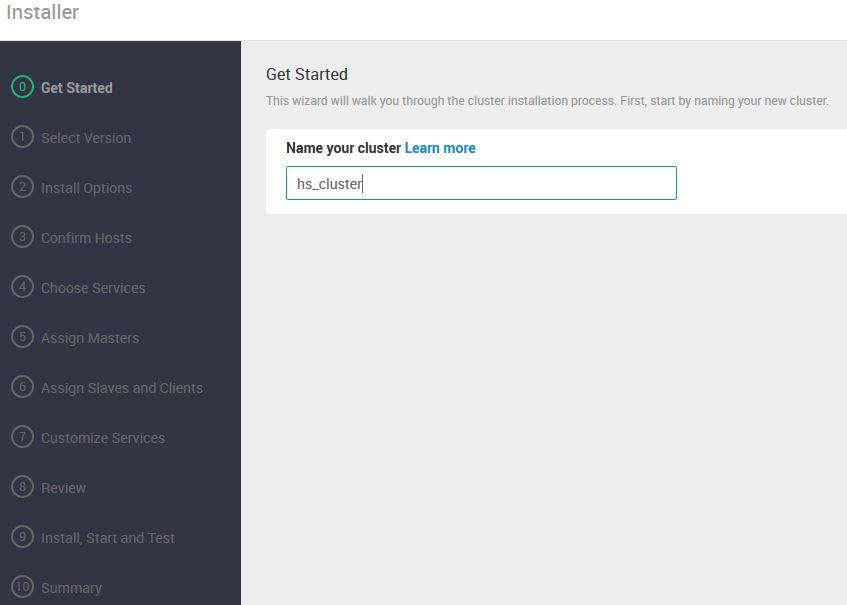
\includegraphics[width=1.3\textwidth]{img/hscluster}
\captionof{figure}{Ambari Wizard Installer}\label{pic:hscluster}
\end{figure}
\noindent Next, we click through the installation routine until the point appears where the cluster nodes are defined. At this point the fact that we are using Ubuntu 18.04 will cause some troubles. If we adding the hosts Ambari is trying to check some dependencies and is running also some check routines. It will fail to add the worker nodes to the cluster since OS is not supported (termination condition). The solution to this problem would be a downgrade of the OS but we don’t have the privileges to do this. So we manually
changed the \textbf{/etc/issue}, \textbf{etc/lsb-release} and \textbf{etc/os-release} file to Ubuntu 16.04 version. Of course, a backup of the original ones has been created as well. After this workaround, the check condition will not fail because Ambari consider our OS as Ubuntu 16.04. Obviously, that’s a dangerous operation, so we change it back to original state after installation has been completed.
In the next step we are choosing our Hadoop services that may be relevant for our data science project. For a start we choose following services: HDFS, YARN, MapReduce2, Tez, Hive, ZooKeeper, Ambari Metrics,
SmartSense, Spark2 and Zeppelin Notebook. Interesting to see is that the proprietary service SmartSense
is the only one that cannot be deselected. We have to install it, even if we don’t want to use it. That’s
certainly not very user-friendly. However, it is simple to add further Apache services on running Ambari
but more difficult to uninstall them so we am do not enable all possible Hadoop services from the
beginning. In addition, some services are not for interest at the moment, hence they would only consume
storage without having a practical effect.\\
After some additional configuration steps we can choose which services should run on master or worker
nodes. Also we have to decide which node should be data node and node manager. In this cluster all four VMs are data nodes as well as node managers. A database connection is also mandatory at this step. Depending on selected services there are several database connections. For instance, the
service Hive needs a working SQL database connection. We can choose between MySQL (MariaDB),
PostgreSQL and Oracle. For a first test, MySQL is used as Hive database. We can change the database
connection setting on Ambari at any time. If the configuration has been finished, a summary with all decisions taken is shown. That’s the last possibility to change a fundamental Hadoop setting. It is worth to check all configurations carefully. Afterwards there is no go back option and the uninstall routine of Ambari is complicated and might lead to tremendous work of removing operations. That is also negative criteria of HDP and Ambari. As soon as the installation completes we can switch to the Ambari monitor. Unfortunately, almost all
selected services were offline or could not start properly. A deeper investigation showed that there were
some permission problems with HDFS and the Hadoop user. The HDFS folder was only for root user but
not for user \glqq Hadoop\grqq. With the command \textbf{chown -R hdfs:hadoop /hadoop/hdfs} the correct permissions could be granted.\\
Another problem was that YARN could not start the name nodes due to connection refused error
messages. As \textbf{netstat -tupln | grep 50070} shown the service was only running for localhost address. After changing the binding address to \textbf{0.0.0.0} on HDFS, the communication between the cluster nodes was working and the name nodes could properly start. However, after fixing this issue, the most services were running. The community of Hortonworks was quite helpful in this case. We got an answer within four hours whereas for getting an answer in Cloudera’s community took three times longer.\\
The data node of the master node was not running correctly. It could be started from Ambari and after
few seconds the data node went offline. A look at the error log of this node showed that the cluster id was already used by another node. Removing the HDFS data folder of the data node solved this issue because
afterwards it generates a new cache file with a new cluster id.\\
The following screenshot shows a (successfully) completed Ambari and HDP installation on our VMs.
\begin{figure}[H]
\hspace{-3.4cm}
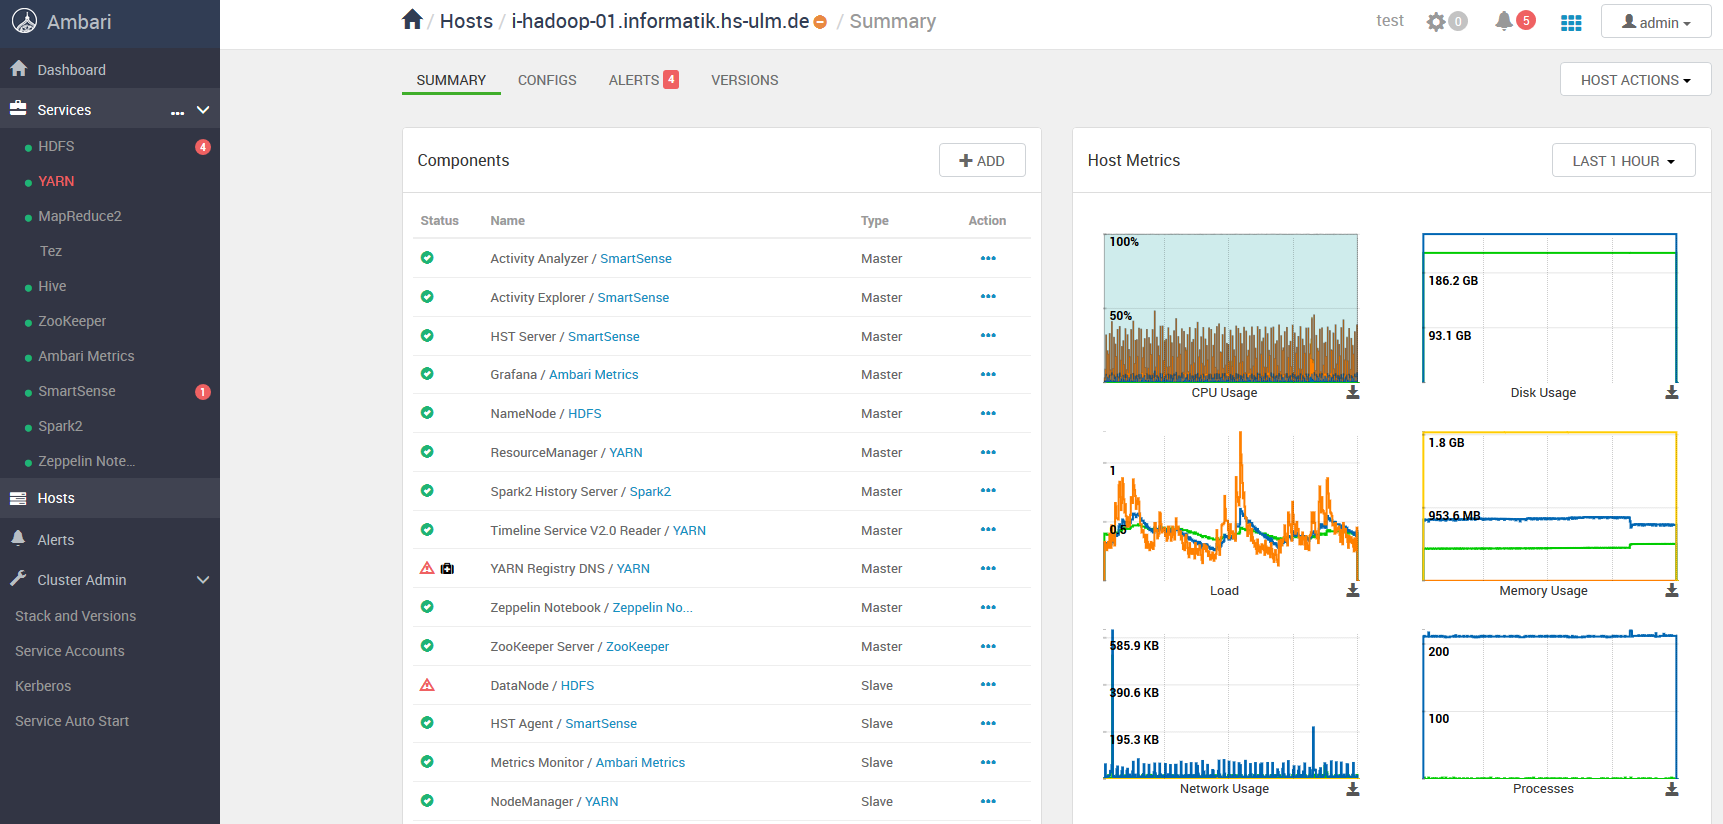
\includegraphics[width=1.5\textwidth]{img/ambari}
\captionof{figure}{Ambari Surface, Host metrics on master node}\label{pic:ambari}
\end{figure}
\noindent Ambari has been set up and most Hadoop services are running (see Figure \ref{pic:ambari}). Ambari shows lot of statistics that might be helpful for cluster management. We can control each service and either turn it off or set it into a maintenance mode. The ladder one encapsulates the service without influencing other services (high availability). Overall, Ambari is a powerful Hadoop cluster management tool that has lot of control options and supervising tools but also lacks in removing services and usability (e.g. no Ubuntu 18.04 support, only Python 2.7.x support, etc). The fact, that there is no official uninstaller from Hortonworks makes HDP with Ambari a risky installation. On the other hand, it is completely open source and has a strong community. Furthermore, HDP 3.0.1 comes up with a bunch of useful Hadoop services and well documentation so that we will likely stay on HDP.\\ Now it is time to run some MapReduce jobs on our newly created Hadoop cluster. 
\subsection{Run MapReduce Jobs}
With four workers (master is also a worker node) a significant speed advantage over single computing should be achieved. First, with a MapReduce job, the accuracy of the decimal places of PI is determined using the quasi Monte Carlo method. This MapReduce job is also offered by the Apache foundation (Source). In the console of the master node the MapReduce job can be started with \acs{yarn} as
follows:
\begin{lstlisting}[language=bash,breaklines=true]
yarn jar /usr/local/hadoop/share/hadoop/mapreduce/hadoop-mapreduce-examples-
3.1.1.jar pi 16 1000
\end{lstlisting}
The \emph{PI job} calculates 16 maps where each map process contains 1000 samples. After a short time, the job is finished and the following output is achieved:
\begin{figure}[H]
\hspace{1.2cm}
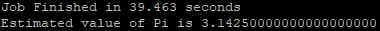
\includegraphics[width=0.8\textwidth]{img/job}
\captionof{figure}{PI Quasi Monte Carlo method executed as Cluster job}\label{pic:job}
\end{figure}
\noindent The same test has been performed with two worker nodes (i.e. two of the four workers were temporarily disabled via Ambari). After that the job took much longer (about 56 seconds). This shows that the Hadoop cluster works and already has a performance advantage over single computing. The next test was a simple WordCount job in Java that calculates the frequency of unique words in an input file distributed across the cluster. A MapReduce job consists of at least a mapper method, a reducer method and a driver method which is often the start method. Before executing the new job one has to put the file of interest on Hadoop’s HDFS. This is simply done as shown below:
\begin{lstlisting}[language=bash,breaklines=true]
hadoop fs -put big.txt
\end{lstlisting}
The put command will upload the file into the HDFS (i.e. it is stored fault-tolerant and replicated 3 times). After that, the following command runs a WordCount job on this text file:
\begin{lstlisting}[language=bash,breaklines=true]
hadoop jar hadoop-mapreduce-examples-3.1.1.jar wordcount wordcountFile big.txt
\end{lstlisting}
Note that now \glqq Hadoop\grqq is used, which starts also the YARN service. There is no difference between executing this with the Hadoop or YARN command. (Although latter is newer and should be used). The output of the \glqq reduced\grqq file looks like figure \ref{pic:words}.
\begin{figure}[H]
\hspace{5.2cm}
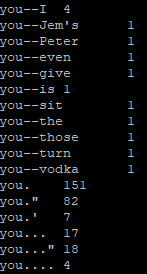
\includegraphics[width=0.2\textwidth]{img/words}
\captionof{figure}{Output of WordCount job}\label{pic:words}
\end{figure}
\noindent Quick to recognize that the words were separated and counted by spaces. In fact, the input text was split
afterwards and each word was mapped as "key value pair", where the key in this case is the word. The
original text file was 6.4 MB, while the newly created file is only 0.93 MB in size. This shows another
potential benefit of the cluster, namely the possible separation of files to minimize the total size of the initial data set. The running time was around 10 seconds. The same job has been executed locally on a
commodity Windows client in NetBeans as well and it took around 8 minutes. There is a plenty of further typical MapReduce jobs (e.g. terasort, randomwriter, sudoko, etc), but for an evaluation these two jobs should already show that the cluster is working apparently faster than a single node.
\subsection{HDP Issues}
Due to the workaround in Chapter \ref{intallhadoop}, a few services could not start properly. Also, permissions for some subfolders were set incorrectly, hence permission denied errors occurred when running the services. During the test phase some other problems were discovered, which are described below. Table \ref{tab:issues} also shows the solution that was found to resolve these issues.
%first part of table issues!
\begin{table}[H]
\hspace{-2.0cm}
\begin{tabular}{|p{4.4cm}|p{12.4cm}|}
	\hline
	\textbf{Issue} & \textbf{Solution} \\ \hline
	No starting NameNodes, Connection
refused. & Go to HDFS$\rightarrow$ Filter at https
0.0.0.0 and \newline localhost address on master node \newline http
127.0.0.0:50070 $\rightarrow$ 0.0.0.0:50070\newline Hive could not start on Node 2 since database was missing (mysql) Permission on HDFS was set to root and not to user hadoop
\\ \hline
Wrong Permissions on HDFS & tail hadoop-hdfs-namenode\newline
chown -R hdfs:hadoop /hadoop/hdfs \\ \hline
Hive Database not found on i-hadoop-02 & \begin{itemize}[noitemsep,leftmargin=*] 
\item Start mysql
\item Show databases;
\item create database hive;
\item CREATE USER 'hive'@'localhost' IDENTIFIED BY 'hive';
\item GRANT ALL PRIVILEGES ON . TO 'hive'@'localhost';
\item CREATE USER 'hive'@'\%' IDENTIFIED BY 'hive';
\item GRANT ALL PRIVILEGES ON . TO 'hive'@'\%';
\item GRANT ALL PRIVILEGES ON . TO 'hive'@'localhost' WITH GRANT OPTION;
\item GRANT ALL PRIVILEGES ON . TO 'hive'@'\%' WITH GRANT OPTION;
\item FLUSH PRIVILEGES;
\end{itemize}
\\ \hline
Bind address in mysql-conf (0.0.0.0): & \begin{itemize}[noitemsep,leftmargin=*] 
\item netstat -tupln | grep 3306
\item Nano /etc/mysql/mysql.conf
\item Change bind-address to 0.0.0.0
\item Systemctl mysql restart
\item Service mysql restart
\end{itemize}
\\ \hline
YARN DNS Server not starting,\newline connection refused & \begin{itemize}[noitemsep,leftmargin=*] 
\item Change Port 53 to other Port
\item Set right permissions on YARN folder
\end{itemize}
\\ \hline
\end{tabular}
%\caption{Issues}
\label{tab:issues}
\end{table}
%second part of tabel issues
\begin{table}[H]
\hspace{-2.0cm}
\begin{tabular}{|p{4.4cm}|p{12.4cm}|}
	\hline
	\textbf{Issue} & \textbf{Solution} \\ \hline
Master Node worker is not starting (Conflicting cluster id) & \begin{itemize}[noitemsep,leftmargin=*] 
\item Stop service
\item sudo wget archive.apache.org/dist/zeppelin/zeppelin-0.8.0/zeppelin-0.8.0-bin-all.tgz
\item sudo tar -xf zeppelin-0.8.0-bin-all.tgz
\item Move interpreter to /usr/hdp/current/zeppelin-server/interpreter/
\item sudo chown -R zeppelin:zeppelin/usr/hdp/current/zeppelin-server/interpreter/
\item Start service
\end{itemize}
\\ \hline
Umask is changing from 0022 to 0002 & \begin{itemize}[noitemsep,leftmargin=*] 
\item sudo gedit ~/.bashrc
\item Add line umask 022
\item Logout and login
\end{itemize}\\ \hline
FAILED [2018-12-0813:36:00.609]\newline java.io.IOException:\newline mkdir of /hadoop/yarn/local/filecache/60\_tmp failed & \begin{itemize}[noitemsep,leftmargin=*] 
\item YARN permissions
\item sudo chown yarn yarn
\item sudo chmod 750 yarn
\end{itemize}
\\ \hline
\end{tabular}
\caption{Problems and solutions of HDP}
\label{tab:issues}
\end{table}
\noindent The described problems and their solutions of table \ref{tab:issues} show that many setting options should be checked carefully during the Ambari installation routine (e.g. if a MySQL database exists). Furthermore, it can be assumed that most of these issues can be explained by the \glqq officially\grqq unsupported operating system version. However, after the fix, all Hadoop services in Ambari had a green status point. 
\subsection{Recommendation}
The evaluation showed that Hortonworks with the Hadoop distribution HDP is best suited for our goals.
Ambari provides an efficient, comprehensive cluster management tool for monitoring and controlling the
Hadoop cluster. In addition, an active community and complete open source freedom can convince more
than its competitors. Although all three Hadoop distributions may have their individual advantages and
disadvantages (see evaluation matrix in figure \ref{pic:matrix}), HortonWorks was able to convince us due to the reasonably good documentation and the easy to follow Ambari installation routine. It should be noted, however, that the Cloudera Manager installation wizard also has good documentation and a comparable installation effort. However, we liked the Ambari interface more than the CDH one. In addition, Cloudera's pricing is not entirely transparent and third-party module integration is rather difficult. For example, since CDH 5.11 there has been a proprietary \glqq data science workbench\grqq service replacing Jupyter and IPython notebooks. HortonWorks, on the other hand, offers Zeppelin notebooks that resemble the famous Jupyter notebooks. Apart from that, Jupyter could also be installed as a third module during the test phase of HDP, even though such installations are naturally risky and are not officially supported by HortonWorks.
\\It is interesting that MapR, HortonWorks and Cloudera offer Docker images for immediate testing. For
example, MapR offers a VMware image free of charge. However, all these packages have the disadvantage
that they only have a single node cluster and limited functionality. For example, I could not select any
services or create new ones in MapR and the function to add more worker nodes to the existing cluster
was also not available. Therefore, such images or sandboxes are ideal for a quick check of the user interface and some standard functions, but rather insufficient for a complete range of functions or a productive system.\\
In conclusion it can be said that all three Hadoop distributions would meet the requirements of a big data
project or our project perfectly, but HortonWorks could simply convince more with the overall score than
the more commercially oriented counterparts. Ultimately, the performance also depends on the hardware
of the individual cluster nodes. Due to a low physical RAM, MapReduce jobs even with MapR's high
performance HDFS would be processed slowly by YARN and would probably lead to
\emph{MemoryOutOfExceptions}. Because Hadoop and every single service on top needs resources and these can
quickly bring a commodity computer with standard equipment to its knees. In any case, the HDP cluster is
ready for big data tasks and will be extremely helpful to us in the further course of the project. With Apache Spark, even better performance values might be achieved due to its \glqq in-memory\grqq engine. The test cluster with the four VMs also showed which special features and requirements you should pay attention to (e.g. operating system version).
\subsection{Hadoop Rollout}
For the Hadoop rollout ten fat clients each with 32 GB RAM and 2 TB HDD as well as 128 GB SSD
have been used. The nodes were connected with a 48port Gigabit switch and a routable gateway,
so that all nodes were in a single local domain. For various reasons (e.g. security) the installation
of a hypervisor (Proxmox) has proven to be successful, with which any number of VMs can be
generated and configured (figure \ref{fig:figure1_proxmox}).
\begin{figure}[H]
\hspace{-2.8cm}
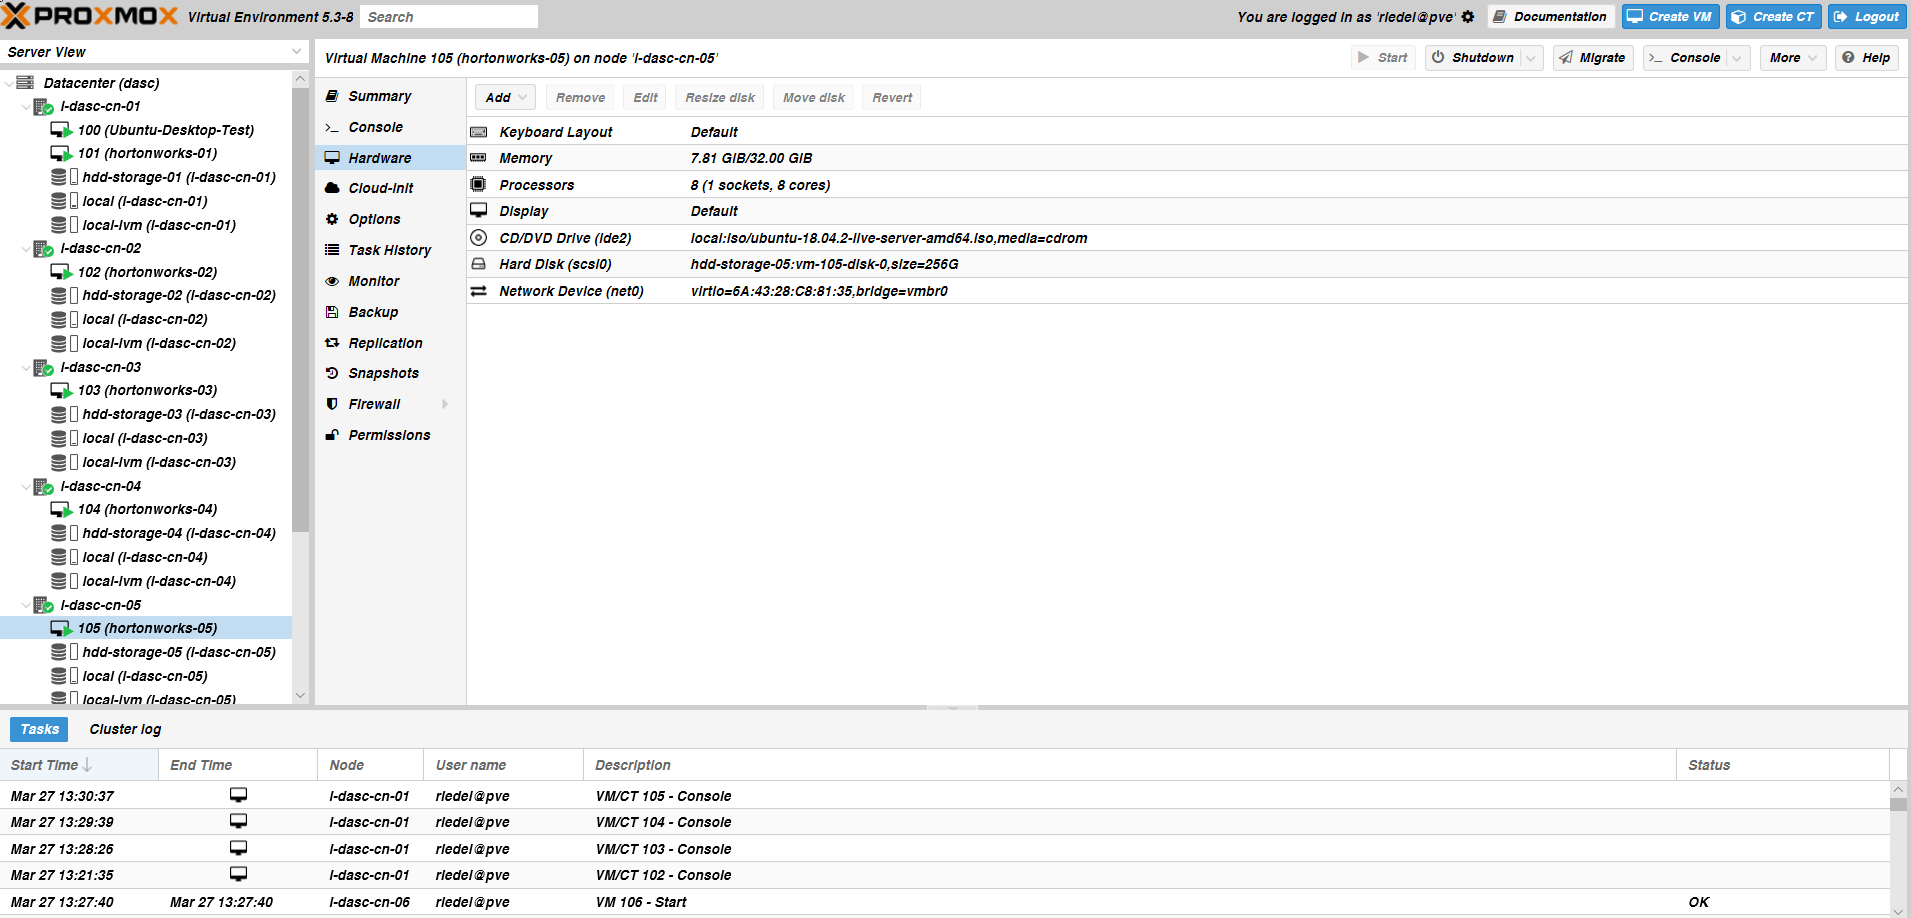
\includegraphics[width=1.4\textwidth]{img/figure1_proxmox}\label{fig:figure1_proxmox}
\captionof{figure}{Proxmox surface}\label{fig:figure1_proxmox}
\end{figure}
A VM with Ubuntu Server 18.04.02 LTS was installed for each node. Each VM got an allocated
memory of 256 GB and a reserved memory for the Logical Volume Manager (LVM). Furthermore,
sparse files were allowed and VirtIO SCSI interfaces were configured for the individual VMs, which
should guarantee maximum VM performance (\cite{RN1}).\\\\
For the first rollout attempt, six cluster nodes were configured for Hadoop. The remaining four nodes
were later added to the existing Hadoop cluster via Ambari surface. The chosen Hadoop stack
was HDP from Hortonworks, as already explain in the Hadoop evaluation part of this work. In
addition, Webmin was installed on the master node, which offers extensive monitoring services
on the node. For example, the current CPU load, memory usage, kernel information and much
more can be displayed. Figure \ref{fig:figure2_webmin} shows the surface of Webmin. Although monitoring services
are also offered with Ambari Metrics, they run on top of Hadoop and can only be called when
Ambari is running as well (\cite{RN2}).
\begin{figure}[H]
\hspace{-3.2cm}
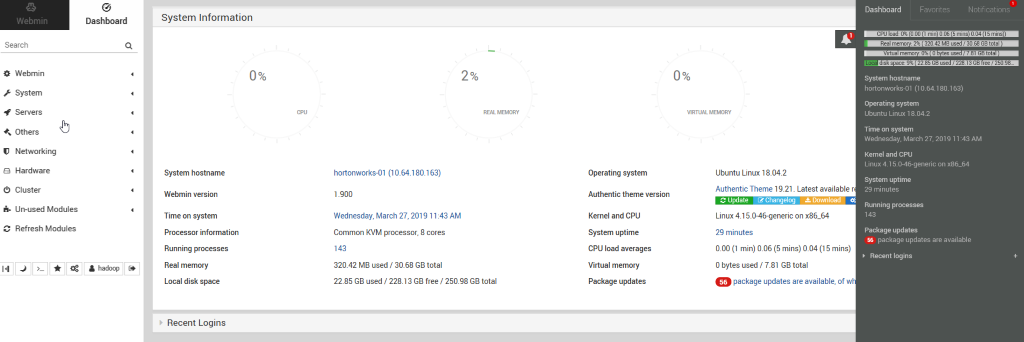
\includegraphics[width=1.5\textwidth]{img/figure2_webmin}\label{fig:figure2_webmin}
\captionof{figure}{Webmin dashboard}\label{fig:figure2_webmin}
\end{figure}
Before the Ambari Wizard can install HDP, some pre-configurations have to be done on each VM.
On the one hand, \glqq ulimit\grqq must be set to at least 10000, because Ambari installs several thousand
dependencies. On the other hand, a password-less ssh authentication is necessary so that the
master node can connect to its worker nodes without entering a password. In addition, the master
node must be able to execute \glqq sudo\grqq commands without entering a password. This can be done
by editing the \glqq visudo\grqq file and adding \glqq username ALL=(ALL) NOPASSWD:ALL\grqq . Another
necessity is to add the IP addresses and hostnames of all cluster nodes under \glqq /etc/hosts\grqq . This
must also be done on each node individually. The following table shows the current host
configurations of a worker respectively slave node:
% vim:ft=tex

\section{Data Profiling}

Data profiling is the process of reviewing source data, understanding structure, content and
interrelationships, and identifying potential for data projects. For the project, the Santander Bicycle data will be profiled more closely \citep{TFL2019}. For this I mainly used Zeppelin notebooks and the HDP cluster with four worker nodes initialized in chapter \ref{intallhadoop}. Zeppelin works similar to Jupyter notebooks and also supports magic commands. However, Zeppelin stores the notebooks in .json format, while Jupyter notebooks (python) uses \textbf{.ipynb}. A corresponding import of Zeppelin notebooks into Jupyter is therefore not possible and
should be considered when working with one of them. Furthermore, as already mentioned, HDP only
supports python 2.7.x, so all Python code in Zeppelin is python 2.7.x as well. (The Nominatim server and
Django already use Python 3.7.x).
\subsection{Data Preparation}
The Santander bicycle data is available on the public Transport for London TfL website.
The structure of these data is as followed:
\begin{itemize}
\item CycleCounters: has information about speed, bike details (length, wheels, axles, class...),
direction, timestamps and serial number.
\begin{itemize}
\item Blackfriars May and June and July
\item Embankment May and June and July
\end{itemize}
\item CycleParking: contains proprietary map material
\item CycleRoutes: contains geographical spatial data (GeoJSON) and .KML files
\item Usage-stats: information about rental stations, duration, start / end time
\end{itemize}
With regard to the folder structure shown above, CycleRoutes and Usage-stats are decisive. In
\glqq CycleCounters\grqq, apart from the maximum driven speed (56 mph!) with a borrowed Santander Cycle, no noteworthy information is contained. Therefore, only the CycleRoutes and Usage-stats data are
considered in the first step of Data Profiling. The CycleParking folder could contain useful map material,
but I only know from Google Earth that can read \textbf{.kml} files and that it is neither compatible with Geopandas nor with Nominatim. Most raw data are available either as .csv files or as .xlsx files.
One problem that arose when reading the usage-stats was that the folder contained 156 csv sheets and
each file was about 30 MB in size. Reading and concatenating as Pandas DataFrame unfortunately
completely occupied the maximum free memory of the master node, so the python job could not be
finished and was in an endless run mode. To work around the problem, we started a Spark job with the
PySpark API on the cluster instead of the Panda DataFrame. The spark job had created a DataFrame from
156 raw files within 12 seconds (i.e. it read 38.122.372 lines of raw text!). What we get here is a so called
Resilient Distributed Dataset (RDD) or Spark DataFrame which, in contrast to the Pandas DataFrame, is
redundant and distributed over the Cluster DataNodes. With the following PySpark method an RDD can
be generated:
\begin{figure}[H]
\hspace{-0.8cm}
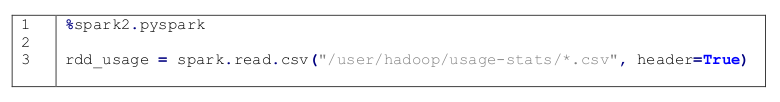
\includegraphics[width=1.1\textwidth]{img/spark1}\label{pic:spark1}
\end{figure}
\noindent Of course the files of the folder \glqq usage-stats\grqq need to be stored on HDFS before it can be read in with Spark. There are several ways of doing this, we used just a Zeppelin cell with magic command shell (\%sh) to execute shell based commands within the notebook. With that one can use:
\begin{lstlisting}[breaklines=true]
execute hdfs dfs -put
/home/hadoop/TFL_Cycling_Data_raw/usage-stats
/user/hadoop/usage-stats
\end{lstlisting}
to push the files on the datanodes of HDP. Remember the default replication size of Hadoop is 3, i.e. the
files are replicated on three worker nodes but not on fur, which should still be resilient enough.
The next decisive step is to prepare the usage-stats data and clean it up a bit. If we read in the data as
described above, our Spark DataFrame has the following columns:
\begin{lstlisting}[language=bash,breaklines=true]
|Rental Id|Duration|Bike Id| End Date|EndStation Id| EndStation Name|
Start Date|StartStation Id| StartStation Name|
\end{lstlisting}
Since we only want to plot the bicycle stations at this time, the Rental ID columns and the date columns
have been removed. This has the advantage that the DataFrame is already smaller and we don't carry any
unnecessary ballast. Furthermore, NaN values have been replaced by mandatory \glqq 0\grqq and duplicates have been removed. The TFL also offers numerous .xml based live feeds, from which we can get the coordinates (longitude and latitude) to the rental stations. We can also use this to fetch the coordinates:
\begin{figure}[H]
\hspace{-0.8cm}
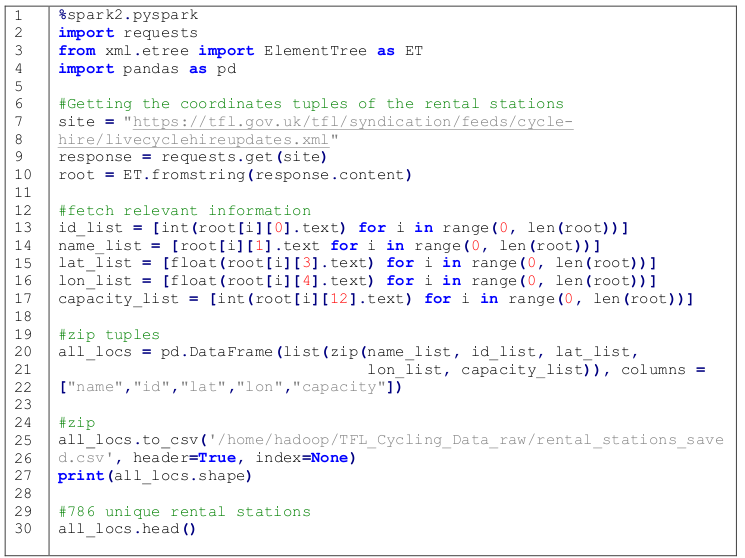
\includegraphics[width=1.1\textwidth]{img/spark2}\label{pic:spark2}
%\captionof{figure}{}
\end{figure}
\noindent This gives us not only the longitude and latitude, but also the maximum bicycle capacity of any station in London. This information could still be quite useful. As you can see, we have 786 unique bicycle stations in London (which are quite a lot).
Remark: Livecyclehireupdates.xml contains also following attributes:
\begin{itemize}
\item installed
\item locked
\item installDate
\item nbBikes
\item nbEmptyDocks
\item nbDocks
\end{itemize}
Given that there are 786 stations across London (at least at the time of writing), this allows for 786 * 785 = 617.010 possible journey combinations if we ignore those that start and end at the same station. The
next step is some data cleansing steps such as sorting, renaming and converting data types. PySpark offers
similar operations for the RDDs as for Pandas DataFrames. However, some pandas such as \glqq iloc()\grqq cannot
be transferred to Spark RDDs. Therefore Spark offers the option to directly execute SQL queries in
DataFrames. Anyway, the fetched data from the live feed must still be merged with the rdd\_usage Spark
DataFrame. For this purpose we first saved the Pandas DataFrame locally and then uploaded it to the
HDFS. This checkpoint is then read in again with PySpark as RDD. Merging works similar to SQL or/and
python. To do this, simply use the \glqq join\grqq command to link the two DataFrames:
\begin{figure}[H]
\hspace{-0.8cm}
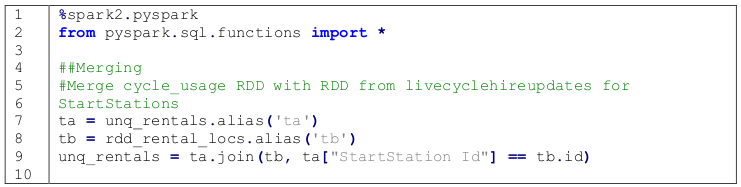
\includegraphics[width=1.1\textwidth]{img/spark3}\label{pic:spark3}
\end{figure}
\noindent In this case we also used alias (similar to the alias of SQL) in order to shorten the joining function name. The rest of the merging stuff is automatically done by the Spark API. After all the data
munging steps we got following schema of our combined and prepared usage-stats table:
\begin{lstlisting}[breaklines=true]
StartStation Id|EndStation latitude|StartStation Id|Duration|StartStation longitude|StartStation
Address|StartStation capacity| EndStation Address|EndStation latitude|EndStation longitude|EndStation capacity|
\end{lstlisting}
One can note, that there are also the columns \glqq StartStation ID Used\grqq and \glqq EndStation ID Used\grqq which stands for frequency of rented bikes on a single station. This gives us an indication of how
popular the station is in comparison with other ones. It might be also used as a weighting factor
for plotting on maps which will be described in just a moment.
With this, we can begin to plot statistics. But at first let compare the size of the new file with the
total size of all loaded cycle-usages. The total size was around 5.4 GB (which could not be simply
loaded into a Pandas DataFrame) whereas the new DataFrame has only 0.9 GB size. The reduction
of the size can be explained by the fact that we removed some unused columns and dropped
duplicates. This means also we are now able to use Pandas because to load 1 GB into a local
memory should be possible for most common computers. In fact, the Hadoop test environment
has shown its functionality and legitimation for the using in big data projects.
\begin{figure}[H]
\hspace{-0.8cm}
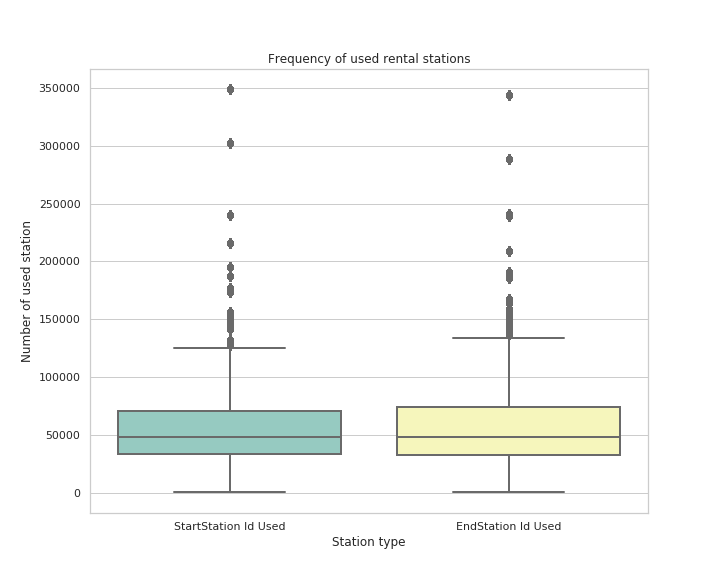
\includegraphics[width=1.1\textwidth]{img/plot1}
\captionof{figure}{Frequency of used StartStations and EndStations}\label{pic:plot1}
\end{figure}
\noindent As we can see from Figure \ref{pic:plot1}, the use of end stations slightly outweighs the starting stations,
which merely means that more different end stations than different start stations
were used. Apparently there are some very popular rental stations like the outliers from figure
\ref{pic:plot1} show. It is worth noting that the data were all collected from 2016 - 2018. (The year 2014-2016 are not included in this case). 
The next plot should serve us to show the density center of the rental stations locations. For this a joint
kernel density estimation plot could be helpful. We are plotting longitude against latitude of each single
StartStation. The illustrations looks then like this:
\begin{figure}[H]
\hspace{-0.8cm}
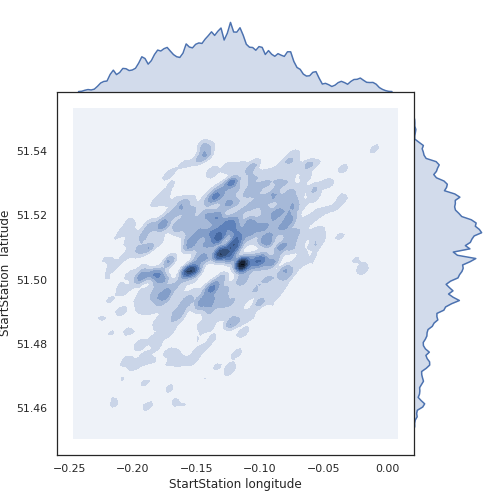
\includegraphics[width=1.1\textwidth]{img/plot2}\label{pic:plot2}
\captionof{figure}{Frequency of used StartStations and EndStations}\label{pic:plot2}
\end{figure}
\noindent 
The centroid or center of this plot is indicated by the dark spots. There are the most rental stations as also the frequency distributions (i.e. histograms) on the right border and on the top are clearly showing. Apart from that center of gravity, on the right corner there are also rental stations placed (guessing between longitude: -0,01 and latitude 51,6) which indicates that these rental stations must be placed in an outer borough of London. At a next, it would be useful to show the rental stations on a map based on their usage. As already mentioned we have 786 unique rental stations so that we can drop the duplicates for this case. In fact, we have saved the number of used stations on a separate column. At this step we prefer to use Jupyter on a local machine since Zeppelin on the cluster is not supporting IPython Display which is required by third-party packages such as folium. So we loaded the prepared cycle-usage data into a local Pandas dataframe. Now we can plot a heatmap for the rental stations:
\begin{figure}[H]
\hspace{-0.8cm}
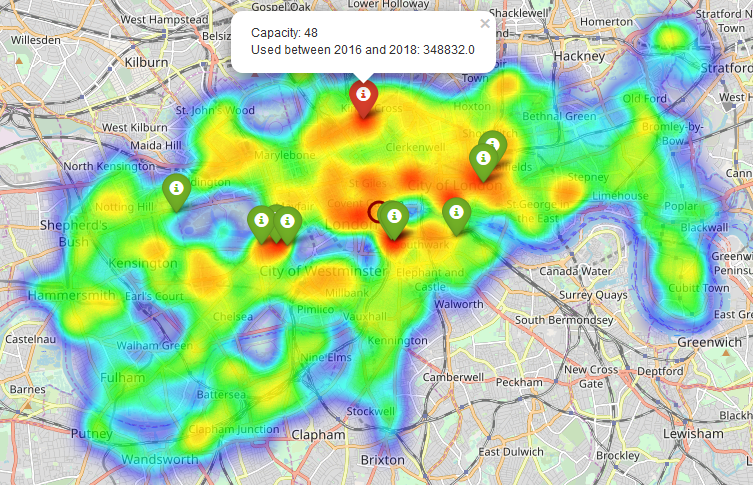
\includegraphics[width=1.1\textwidth]{img/heat}\label{pic:heat}
\captionof{figure}{Top 10 used Santander rental stations}\label{pic:heat}
\end{figure}
\noindent 
The red marker in figure \ref{pic:heat} indicates the most often used bicycle station in London in last two years. This is not surprisingly because close to the biking station there is London train station. Probably many travelers who are arriving by train are using a Santander cycle. However, this interactive map has been saved and uploaded on a webserver on the Hadoop cluster (\href{http://i-hadoop-01.informatik.hs-ulm.de/most_stations.html}{link})
As we can see, there are many rental stations close together. For a first impression this should be enough
as one can already see the capacity of each single Santander rental bike station by clicking on the marker
and also the location of each station is visible on the map. As an addition one can see the frequency of
each station by looking at the sizes of the heat spots or/and reading marker details.
\subsection{Conclusion of the file sizing problem}
\begin{enumerate}
\item The sizing problem can be well handled by Spark
\item The HDP is working and storing the cycle-usage files on HDFS
\item For plotting tasks packages like folium or seaborn cannot be used with Spark DataFrame
\begin{itemize}
\item Converting back to Pandas DF might exceed local RAM
\item Using Jupyter notebook on local computer for plotting maps (e.g. folium)
\end{itemize}
\end{enumerate}
\subsection{CyclingRoutes}
The Cycling routes from the folder of TFL [24] are geojson files and represent real geographical
routes within London inner city.
There are 5 \emph{geojson} files in this folder available:
\begin{itemize}
\item \emph{Central\_London\_Grid.json}
\begin{itemize}
\item \emph{Central London Grid}: i s a set of safer, connected routes for cyclists across central London
\end{itemize}
\item \emph{Mini\_Hollands.json}
\begin{itemize}
\item Mini-Hollands have features that make cycling feel safer and more convenient.
\end{itemize}
\item \emph{Quietways.json}
\begin{itemize}
\item \emph{Quietways} are signposted cycle routes, run on quieter back streets to provide for those cyclists who want to travel at a more relaxed pace.
\end{itemize}
\item \emph{super-highways-quietways.json}
\begin{itemize}
\item \emph{Combination of super highways and quietways}
\end{itemize}
\item \emph{Cycle\_Superhighways.json}
\begin{itemize}
\item \emph{Cycle\_Superhighways} are on main roads and often segregate cyclists from other
traffic.
\end{itemize}
\end{itemize}
The routes should be concatenated by a single GeoPandas GeoDataFrame. Doing so requires to read the
geojson files with following scripts:
\subsection{Plotting Data}
Let’s see if we can compare the frequency of used rental stations between StartStation and EndStation.
We can not use swarm plots or any other kind of plots with fine granular details since \glqq matplotlib\grqq or Python would try to draw over six million dots which will easily exceed the local RAM of the master node. Beside from that, we also would see to many points at the same location since lot of stations are drawn several times. A better plot in my opinion is to use a box plot as following figure shows:
\begin{figure}[H]
\hspace{-0.8cm}
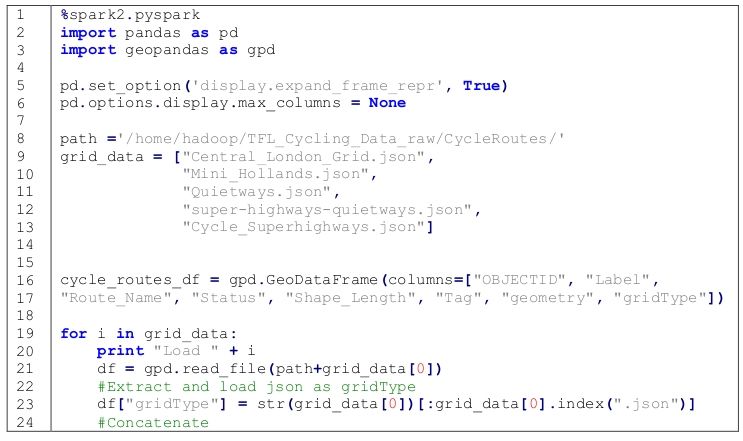
\includegraphics[width=1.1\textwidth]{img/spark4}\label{pic:spark4}
\end{figure}
\begin{figure}[H]
\hspace{-0.8cm}
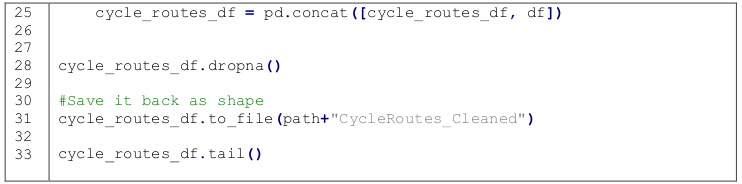
\includegraphics[width=1.1\textwidth]{img/spark5}\label{pic:spark5}
\end{figure}
\noindent So we get in only GeoPandas DataFrame which contains the 5 Cycling routes. In addition, the type of each route was stored in the column \glqq gridType\grqq, so that it can be filtered later for certain routes. For a first plot a Choropleth should show the different routes.
\subsection{Conclusion}
\begin{enumerate}
\item The data lacks in documentation and quality (Data Preperation \& Cleansing necessary).
\item Some column names can be misunderstood (e.g. SITE\_NUMBER <> SITE\_ID).
\item Data like SPEED or SPEED\_MHP should be stored in one way.
\item Many columns like the axles are not meaningful and useful for our project. (e.g. Cyclecounters
has 107 columns!)
\item Raw data seems not to be complete (e.g. only May, June, July)
\item \emph{usage-stats} is very big. Necessity to use all usage-stats?
\end{enumerate}
In the next sprint we will create similar plots as shown above, but this time with duplicates and times in mind. Because it is quite often the case that between two same bicycle stations several same entries exist at different times with different rental periods. For example, a use case would be to display the day/night change on the map,
i.e. do more cyclists ride quietways or super-highways at night between rental stations?

% vim:ft=tex
\section{Prediction on Daily Basis}\label{sec:daily}
\subsection{Data Profiling Part II}\label{dp2}
As already indicated in Data Profiling Part 1 in chapter \ref{dp1}, the next step is to display the use of the routes at
different times between the individual bicycle stations on a map. Since the Python package
"folium" uses leaflet maps based on Javascript \cite{RN5}, the plotting of the routes on an hourly level is
not performant, because too many poly lines have to be drawn and the map can no longer be
efficiently displayed in the browser. Therefore only the top 10\% most used routes were plotted on
the folium map. Another restriction was the aggregated granularity on a daily base. This means
that the plotted map always showed the route usage for day x. With the folium plugin
\glqq TimestampedGeoJson\grqq time series data can be plotted in JSON format. An excerpt from the
script \glqq Cycleusage \& Cycleroutes [allStations].ipynb\grqq shows the corresponding function call:
\begin{figure}[H]
\hspace{-1.6cm}
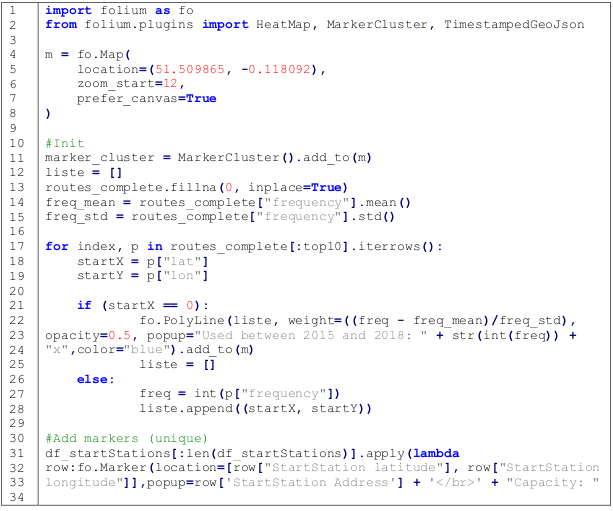
\includegraphics[width=1.2\textwidth]{img/listing1}\label{fig:listing1}
%\captionof{figure}{Result of \acs{mlp} with MinMaxScaler}\label{fig:listing1}
\end{figure}
\begin{figure}[H]
\hspace{-1.6cm}
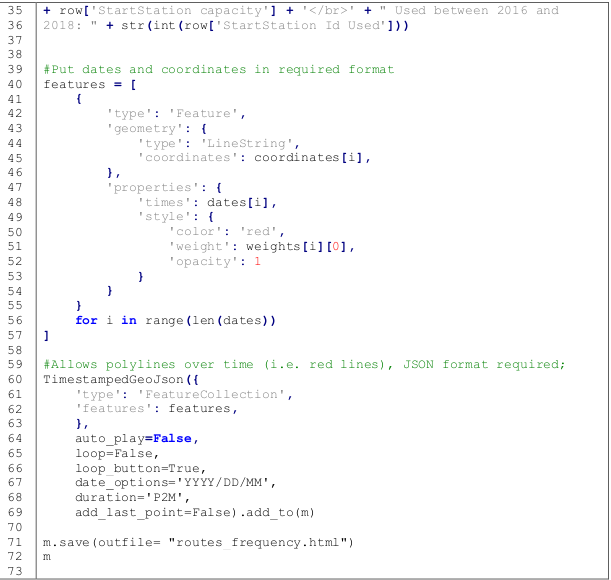
\includegraphics[width=1.2\textwidth]{img/listing2}\label{fig:listing2}
\captionof{figure}{Route usage over time plot}\label{fig:listing2}
\end{figure}
As the code from figure \ref{fig:listing2} shows, the poly lines on the map have been added iteratively. The
weight parameter can be used to determine the thickness of the poly line. Since these should look
as dynamic as possible on the map, the weight has been standardized. The fixed stations were
initially added, but no duplicate stations were plotted. A disadvantage of the plugin is that it needs
the data in a JSON format. Therefore the coordinates for the single points of a poly line as well as
the time series data had to be converted into a compatible format. As can be seen from the Python
code, the coordinates must be given the type \glqq LineString\grqq.  A LineString is defined as a sequence
of uniquely assignable points. In this case, the longitude and latitude previously requested using
the Graphhopper API on our Graphhopper server were sufficient. It is important that the parameter \glqq date\_options\grqq in \glqq TimestampedGeoJson\grqq corresponds exactly to the date format as in the nested
list dates, otherwise the time slider function on the map will not work properly.
Applied to the bicycle data the following picture results for the time 26.06.2016:
\begin{figure}[H]
\hspace{-1.6cm}
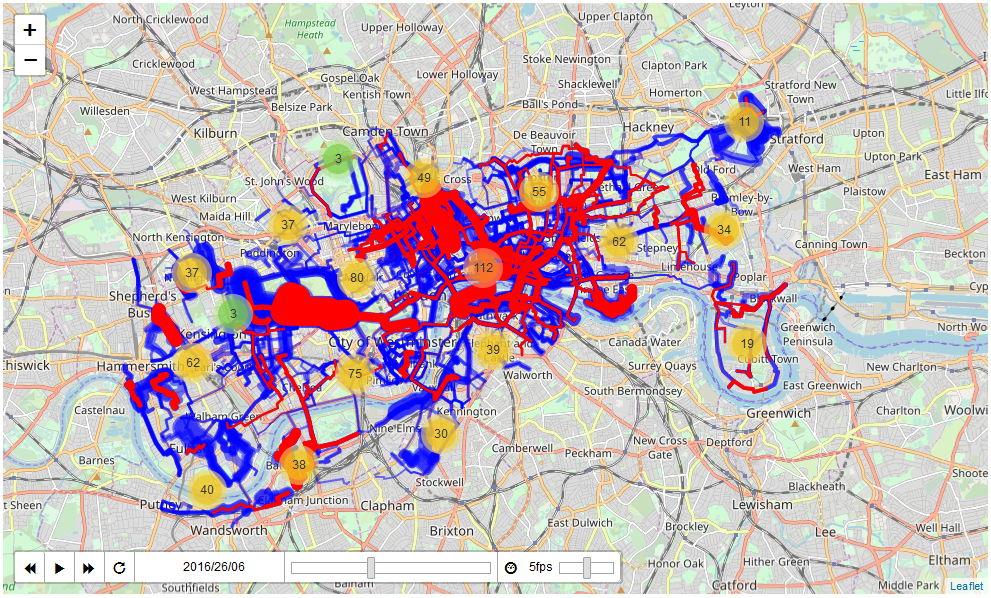
\includegraphics[width=1.2\textwidth]{img/figure4_folium_plot1}\label{fig:figure4_folium_plot1}
\captionof{figure}{Used bicycle routes over time plot}\label{fig:figure4_folium_plot1}
\end{figure}
From figure \ref{fig:figure4_folium_plot1} it can be seen that on this day there was a moderate use of Santander Bicycles in
inner London. Especially the hubs such as Kings Cross or Hyde Park were obviously used very
often with Santander Bicycles on this spring day. Furthermore, the map with the thickness of the
poly lines shows how often this route was used in relation to the total use of all routes. The red
colored routes from figure \ref{fig:figure4_folium_plot1} are the actually used routes on this particular day, while the blue
routes are the \glqq inactive\grqq ones. The bubbles with the numbers represent the respective rental
stations. These have only been aggregated to provide a clearer representation. If the map is
zoomed in (figure \ref{fig:figure4_folium_plot1}), the granularity is refined and the markers of the individual rental station
locations are displayed. The color of these bubbles correlates with the number of aggregated
stations in the vicinity. This method also has the advantage that it is easy to see where most rental
stations are located. In fact, with 112 stations (see figure \ref{fig:figure4_folium_plot1}), the inner districts connected by the
Waterloo Bridge and the London Blackfriars Bridge form the center of most stations which are
close by. It should be noted, however, that new rental stations are constantly being added (even
given up again!), and a new data extract could result in a different picture. Therefore this assumption is valid for the selected date from figure \ref{fig:figure4_folium_plot1}, but not for today or in two years. A useful
feature that comes along with the folium plugin is the automatic data display sequence \cite{RN5}. When
someone clicks on the \glqq Play\grqq button from figure \ref{fig:figure4_folium_plot1}, all time series data is automatically run through.
The speed can be adjusted with the \glqq fps\grqq slider.
To give a counterexample, the following map shows the use of the routes on a winter’s day:
\begin{figure}[H]
\hspace{-1.6cm}
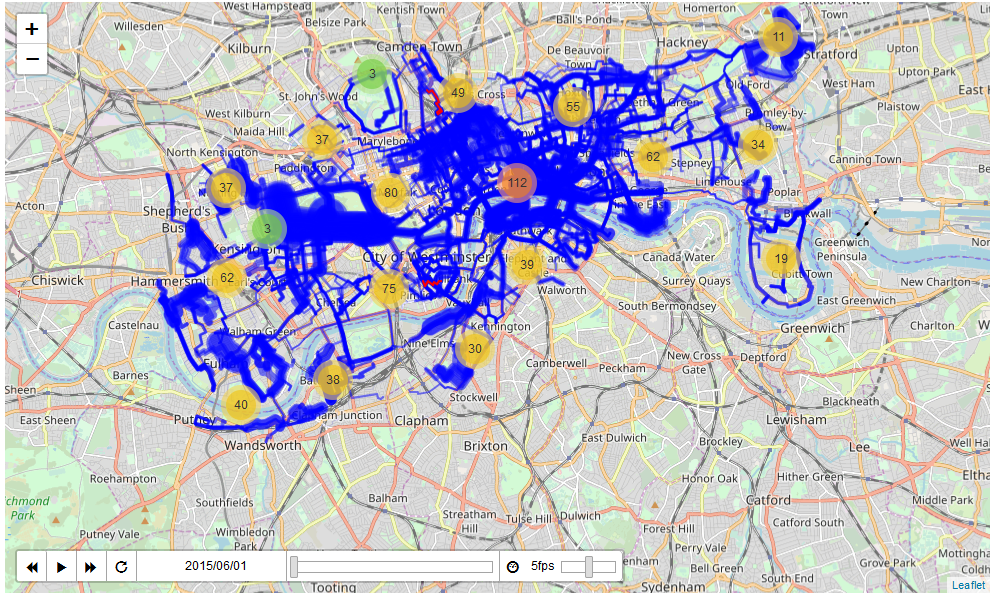
\includegraphics[width=1.2\textwidth]{img/figure5_folium_plot2}\label{fig:figure5_folium_plot2}
\captionof{figure}{Used bicycle routes over time plot}\label{fig:figure5_folium_plot2}
\end{figure}
On 06.01.2015 obviously less bicycles were rented than in figure \ref{fig:figure4_folium_plot1}. This is due to the fact that at
this time it was winter and on the other hand there were only 315 Santander bicycle rental stations
all over London \cite{RN6}. In the course of time, new stations were added again and again, resulting in
a network which is monitored and managed by the local government and administrated by TfL.
The interactive map is also available on the \href{http://i-hadoop-01.informatik.hs-ulm.de/routes_frequency.html}{Hadoop Cluster}.
Overall, it can be observed that the usage of the rental stations has risen sharply on average over
the last four years. This can be explained by the expansion of the network but also by the increased
environmental awareness of the citizens. It is to be expected that further stations will be connected
in the future, so that ideally there will be one rental station at each crossroad in the town.
\subsection{Feature Engineering Kings Cross}\label{king}
Next, the features for the most frequently used station (Kings Cross) were prepared and
aggregated on a daily basis. In addition, these features have been extended by more like
\emph{Holidays, Weekdays, Months, Seasons} and weather data. This enrichment of the features
should help to achieve a higher accuracy of the learning model. For the weather data the weather
API \glqq Dark Sky\grqq was used. Like every available weather API the free use is limited. In the case of
Dark Sky a maximum of 1000 API request calls per day can be executed with one key \cite{RN7}.
However, this limitation can be bypassed if multiple accounts are used. Since each account has
a key, the keys can be collected and thus in fact significantly more requests can be executed.
However, this cannot be applied to the existing data sets of the bicycle data, since the daily
aggregated data of Kings Cross alone has already 376625 rows. Therefore a \glqq dates\grqq file was
created, which contains all days from 04.01.2015 - 14.04.2019 and thus covers all possible date
values of the rental station data. This has the advantage that now only 1562 API requests are
necessary and two keys are sufficient. The disadvantage of this method is that of course no precise
weather data can be retrieved at every station. Therefore the coordinates for the weather data of
the centroids (51.509865,-0.118092) of London were chosen. Dark Sky API also returns a JSON
file as response, which can be searched for the desired information. The following function from
the script \glqq Cycleusage \& Cycleroutes [allStations].ipynb\grqq shows the corresponding request call:
\begin{figure}[H]
\hspace{-1.6cm}
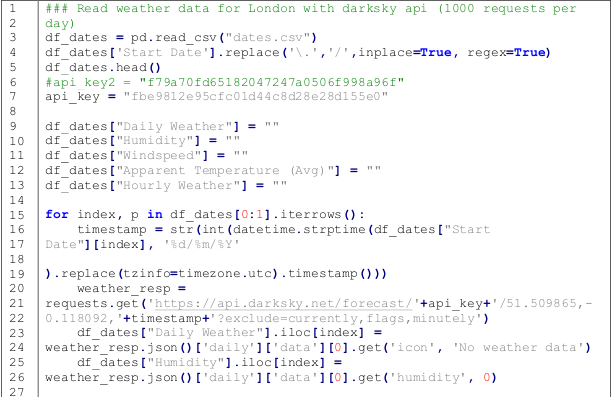
\includegraphics[width=1.2\textwidth]{img/listing3}\label{fig:listing3}
%\captionof{figure}{Result of \acs{mlp} with MinMaxScaler}\label{fig:listing1}
\end{figure}
\begin{figure}[H]
\hspace{-1.6cm}
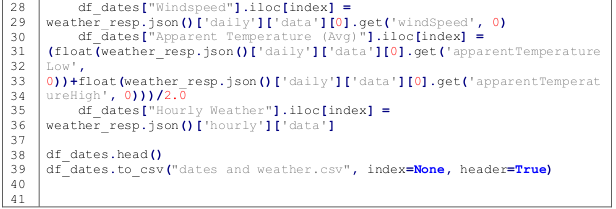
\includegraphics[width=1.2\textwidth]{img/listing4}\label{fig:listing4}
\captionof{figure}{Fetching the weather API with Python}\label{fig:listing4}
\end{figure}
As the code from figure \ref{fig:listing4} clearly shows, the following weather data were considered as relevant:
\glqq Daily Weather, Humidity, Windspeed\grqq and \glqq Apparent Temperature (Avg)\grqq . The feature \glqq Daily
weather\grqq returns a string value, how general the weather was on that particular day (e.g. sunny,
partly-cloudy...). Dark Sky makes this value dependent on the worst condition that occurred on
that day \cite{RN7}. That is, if it snowed for an hour, but the rest of the day was cloudy, \glqq Daily Weather\grqq will still show \glqq snowy\grqq  because this condition is weighted higher.\\\\
In addition to the weather data mentioned above, the hourly weather data of each day was also
queried as JSON lists, as otherwise every hour of each day would have to be queried separately,
which would drastically increase the API calls. A drawback of this variant is that the dates and
weather dataframe has a mixed structure. While the column \glqq hourly weather\grqq is a JSON format,
the other columns have a normal structure. This problem is further addressed in the section \glqq Data
Preparation - Hourly Base\grqq .\\\\
The processed weather data were next merged with the processed cycle usage dataframe. For
the Holidays the Python package \glqq holidays\grqq was used, which returns the corresponding holidays
to a selected location. Similarly, the features \emph{Weekdays, Months} and \emph{Seasons} were be
generated with defined functions and afterwards merged back with the main dataframe.\\\\
Subsequently, the dataframe was supplemented by \glqq past\grqq and\glqq future\grqq data. This should improve
the training of regression models, for example. A kind of \glqq sliding window\grqq was implemented for
the past data. This means that these columns always contain the value of the previous day. With
the future usage data, the daily number of borrowed bikes of the next day was also displayed. The
column \glqq Rented Bikes\grqq (i.e. usage) corresponds to the class variable of interest. This has the
consequence that the first and last day in the dataframe have missing values, because there is no
data for this naturally. The prepared dataframe for Kings Cross on a daily basis looks after the
preparation steps like this:
\begin{figure}[H]
\hspace{-2.8cm}
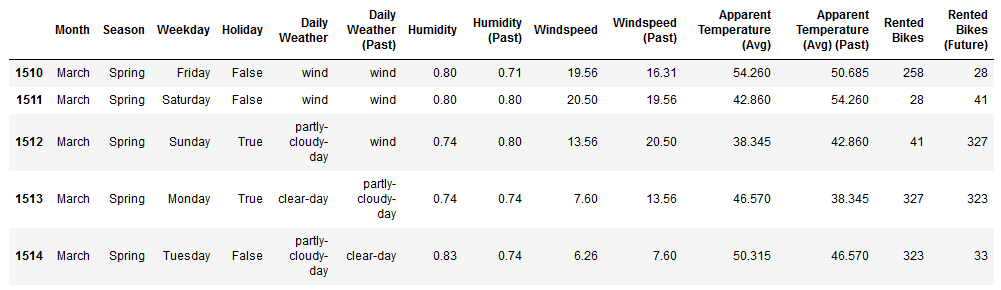
\includegraphics[width=1.4\textwidth]{img/figure6_kings_cross_df}\label{fig:figure6_kings_cross_df}
\captionof{figure}{Prepared data frame of Kings Cross (daily)}\label{fig:figure6_kings_cross_df}
\end{figure}
As one can see from figure \ref{fig:figure6_kings_cross_df}, the past data was only included for the weather data whereas the
future data was only added for the usage of the rental station. The string values were later be
transformed into numerical values since machine learning methods always require number values
instead of string values. Therefore a proper schema was defined, which is described in more detail
in the modeling section.\\\\
With the processed bicycle data from \ref{fig:figure6_kings_cross_df}, machine learning can already be used to predict,
for example, the daily usage of bicycles (i.e. how many bicycles will be borrowed tomorrow starting
from today?). The script \glqq Feature Engineering Kings Cross.ipynb\grqq contains the preparation
functions described above and can be found on our GitHub repository.
\subsection{Data Prediction with MLPRegressor}\label{sec:mlp}
Since we wanted to implement the prediction algorithm in Python we used the library \emph{Scikit Learn} which provides a class \emph{\acf{mlp}} with according functions.
As we wanted to train a non-linear model we decided to use a Multi-layer Perceptron since it can learn a non-linear function approximator for either classification or regression. However  the \acs{mlp} uses backpropagation which is the most widely used algorithm for supervised learning with multi-layered feed-forward networks \cite{riedmiller1993direct}, this algorithm was implemented to train a prediction model for the rental bike usage on a daily base.\\\\
The outcome of of the Data Profiling Part 2, as described in chapter \ref{sec:dp2} served as a basis for the prediction.
As a first implementation we used the following data as an input for the feature matrix: \emph{Month, Weekday, Day, Season, Daily Weather, Daily Weather Past, Humidity, Humidity Past, Windspeed, Windspeed Past, Apparent Temperature (Avg), Apparent Temperature (Avg) Past, Rented Bikes}. Since we assume that weather conditions play an important role in bike usage we decided to add weather data. Another assumption was that on weekdays the frequency will rise, because a lot of people use rented bikes to travel to work. Furthermore we added the number of rentals of today in order to predict the ones of tomorrow. Therefore \emph{Rented Bikes Future} served as our target variable which is to predicted.\\
Since the \acs{mlp} works with data represented as dense and sparse numpy arrays of floating point values, data had to be encoded accordingly beforehand. Therefore we mapped all of the ordinal scaled data like \emph{Month, Weekday, Season, Daily Weather} to numerical data, by implementing a dictionary which assigns numerical values to ordinal data. E. g. For the weekdays we used the following dictionary:
\begin{lstlisting}[language=bash,breaklines=true]
"Weekday": {"Monday": 1, "Tuesday": 2, "Wednesday": 3, "Thursday": 4,"Friday": 5, "Saturday": 6, "Sunday":7 }
\end{lstlisting}
After the encoding we split the data into 80 \% training data and 20\% test data.
Since the \acs{mlp} is sensitive to feature scaling we normalized the data accordingly to the activation function. Since we used the \emph{logistic} activation function which expects values between [0,1] we normalized the feature matrix as well as the target variable beforehand. Scikit Learn provides several scaling mechanism to rescale the data. 
After data was scaled we applied the \acs{mlp} with \emph{logistic} as an activation function and ten hidden layers with five neurons. After the prediction we denormalized the data back to its original state. In order to rate the accuracy of the prediction we computed the \acf{rmse} which measures the difference between actual and predicted values of a model. The less the difference respectively the value, the better is the model.
To get a better impression of how the prediction worked, the results were plotted as time series.
The time series was plotted over for years, which causes the plot to be very large. In order to make it more user friendly, we implemented an interactive plot which gives the user the opportunity to zoom into specific parts or cut out some parts to look at them more closely.
\subsubsection{Normalization}\label{sec:normalization}
In the first attempt we used the \emph{MinMaxScaler} which rescales the data such that all vales are in the range of [0,1].
This gave us a \acs{rmse} of 122.347. To get a better impression of what that means we plotted this result which can be seen in figure \ref{fig:mlpquantile}.
\begin{figure}[H]
\hspace{-2.8cm}
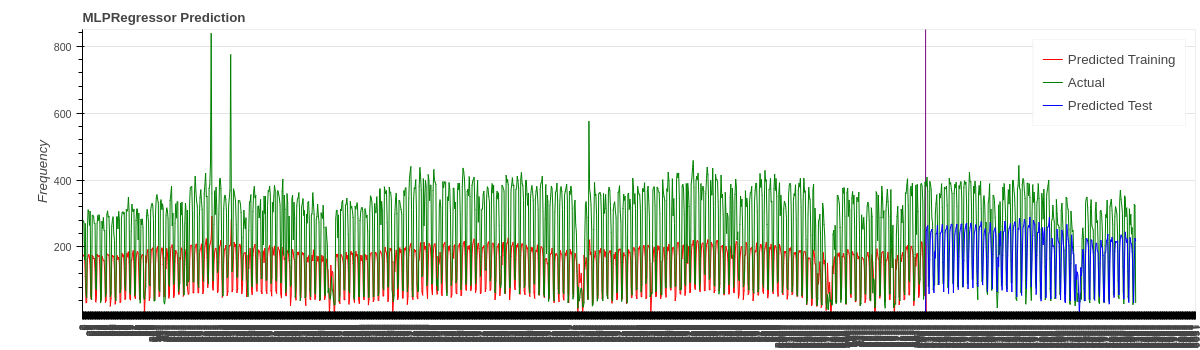
\includegraphics[width=1.4\textwidth]{img/mlpminmax}\label{fig:mlpminmax}
\captionof{figure}{Result of \acs{mlp} with MinMaxScaler}\label{fig:mlpminmax}
\end{figure}
This result shows that the prediction lack accuracy. As we found out this was caused by the MinMaxScaler, since this scaler is very sensitive to the presence of outliers. Therefore we chose another scaler for normalization which is more prone to outliers. In order to find a more suitable scaler, experiments were made with all available scalers of Scikit Learn which met the requirements for the output of the scaling. The best result was achieved by the \emph{QuantileTransformer} with a \acs{rmse} of 57.837, therefore we stuck with this normalization method.
\subsubsection{Feature Evaluation}\label{sec:featureeval}
In order to improve accuracy, further experiments were carried out to evaluate the features. As mentioned earlier the previous predictions were made with a feature matrix of thirteen features. To evaluate which features improve the prediction and which are useless 18 test cases were carried out. Each test case consists of different constellations of features. In the end the different \acs{rmse} values were compared, which can be seen in figure \ref{fig:evalmlp}.
\begin{figure}[H]
\hspace{-1.5cm}
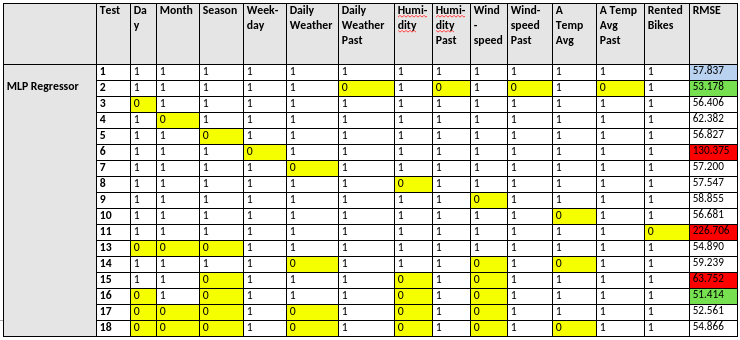
\includegraphics[width=1.2\textwidth]{img/evalmlp}\label{fig:evalmlp}
\captionof{figure}{Feature evaluation test cases}\label{fig:evalmlp}
\end{figure}
Figure \ref{fig:evalmlp} shows beneath the different test cases, included features, those are assigned to \glqq 1\grqq
 and excluded features which are assigned to \glqq 0\grqq. The first \acs{rmse} value, colored in blue depicts the prediction accuracy with all 13 features. The red colored values show the constellations which are significantly worse than the original one and in turn the green values represent the values with an increased accuracy than the original one.
\subsubsection{Result}\label{sec:resultmlp}
This evaluation showed that the features \emph{Weekday} and \emph{Rented Bikes} are the most important ones and in turn the features \emph{Day} and \emph{Season} are less important.
Based on our testing results we recommend to use the following nine features: \emph{Weekday, Month, Past Data, Apparent Temperature (Avg), Daily Weather} and \emph{Rented Bikes}. 
Moreover experiments with scalers showed that the \emph{QuantileTransformer} is more prone to outliers than others and is therefore the scaler of choice.\\
First plots were made with the library \emph{Matplotlib} which turns out to be very restricted and complicated to handle in order to create interactive plots. Therefore we recommend to use \emph{Bokeh} which provides easy to implement interactive plots especially for large data sets.\\
Applying the recommendations regarding scaling and feature evaluation we received a \acs{rmse} value of 51.414 which is the best value achieved during the project phase. The overall result visualized with \emph{Bokeh} can be seen in figure \ref{fig:mlpquantile}.
\begin{figure}[H]
\hspace{-2.8cm}
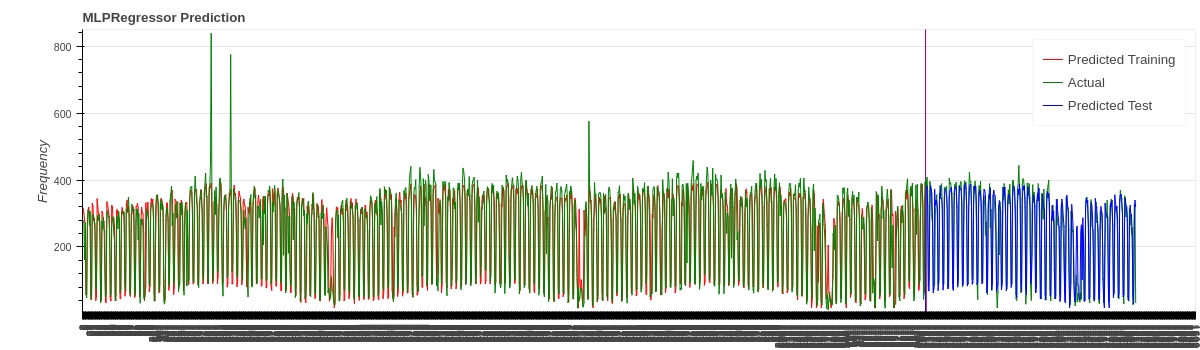
\includegraphics[width=1.4\textwidth]{img/mlpquantile}\label{fig:mlpquantile}
\captionof{figure}{Accuracy with recommended features and scaling by the QuantileTransformer}\label{fig:mlpquantile}
\end{figure}
Compared to figure \ref{fig:mlpminmax} one can see significant improvements in accuracy.\\
This model is based on the most used station, which is King´s Cross with a dataset of 1515 records. In order to confirm this model we applied it to the least used station in Farringdon Street, Holborn as well. The result can be seen in figure  \ref{fig:mlpquantile_least}.
\begin{figure}[H]
\hspace{-2.8cm}
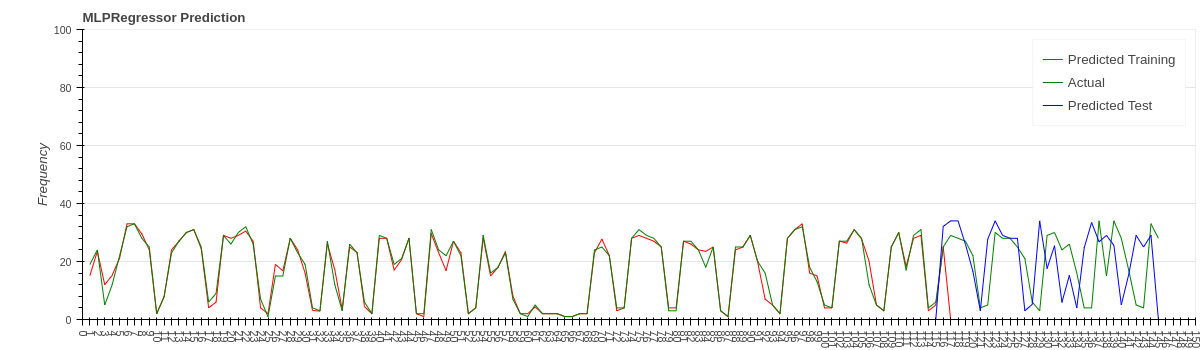
\includegraphics[width=1.4\textwidth]{img/mlpquantile_least}\label{fig:mlpquantile_least}
\captionof{figure}{Accuracy with recommended features and scaling by the QuantileTransformer}\label{fig:mlpquantile_least}
\end{figure}
The accuracy of the prediction of the least used station measures a \acs{rmse} of 9.311. This shows that the model works not only for highly frequented stations but also for stations like Farringdon Street with only 145 records.
\subsection{Modeling (Polynomial Regression)}\label{poly}
Since we don't have a linear relationship between the data, a linear regression will not be helpful.
For example, the regress \glqq Rented Bikes\grqq is not a linear correlation of temperature as even on rainy
days there is slight chance that more people rent a bike than on a sunny day due to a special
holiday. Therefore polynomial regression was a selected machine learning method for the
prediction of rented bikes on a station.\\\\
Polynomial regression belongs to the regression forms \cite{RN9}. In fact, it is just a modified version of a
linear regression. This means the independent variable x and the dependent variable y is modeled
as an nth digress (so-called polynomial) in x \cite{RN9}.\\\\
In a more formal way, the polynomial regression can be expressed as following:
$$Y=\beta_0+\beta_1* x+\beta_2 * x^2 + \beta_3 * x^3 + ... + \beta_n * x^n$$
Where n is the degree of the regression.\\\\
With the Scikit-library in python a data scientist can import the function \glqq PolynomialFeatures\grqq from
\glqq sklearn.preprocessing\grqq which transforms linear data into higher dimensional data. For example
one could apply \glqq poly = PolynomialFeatures(degree = 3)\grqq to get a polynomial
regression in the third dimension. This should improve the accuracy as our underlying data has
no linear relationships but maybe higher dimensional ones. Furthermore, the higher the degree
the better the accuracy should be. Unfortunately the computation time is exponential. A degree of
4 already took several hours to perform and was only slightly better than a regression in the third
dimension.\\\\
The RMSE error on a degree of 4 was around 48,4, which is in comparison to the other tested
ones not really bad but maybe also not best one.\\\\
Figure \ref{fig:figure9_polynomial_features} shows the different plots of each feature and the prediction (rented usage). It turns out
that the feature Season, for example, has no German influence on the use of bicycles, whereby
there was apparently an outlier in spring with 800 rented bicycles. It is also becoming apparent
that bicycles are rented more frequently at low wind speeds than at high wind speeds. The average
temperatures between 30 and 70 Fahrenheit are particularly high. Unfortunately, the addition of
the past data has not caused much change in accuracy, as shown in figure \ref{fig:figure9_polynomial_features}.\\\\
Figure \ref{fig:figure10_polynomial_prediction} shows a plot of the tested data (prediction) with the feature \glqq Daily Weather\grqq . The plot looks relatively good, except for a few single outliers at 2 (partly-cloudy-day), the prediction of the
tested data matches the training data.
\begin{figure}[H]
\hspace{-2.8cm}
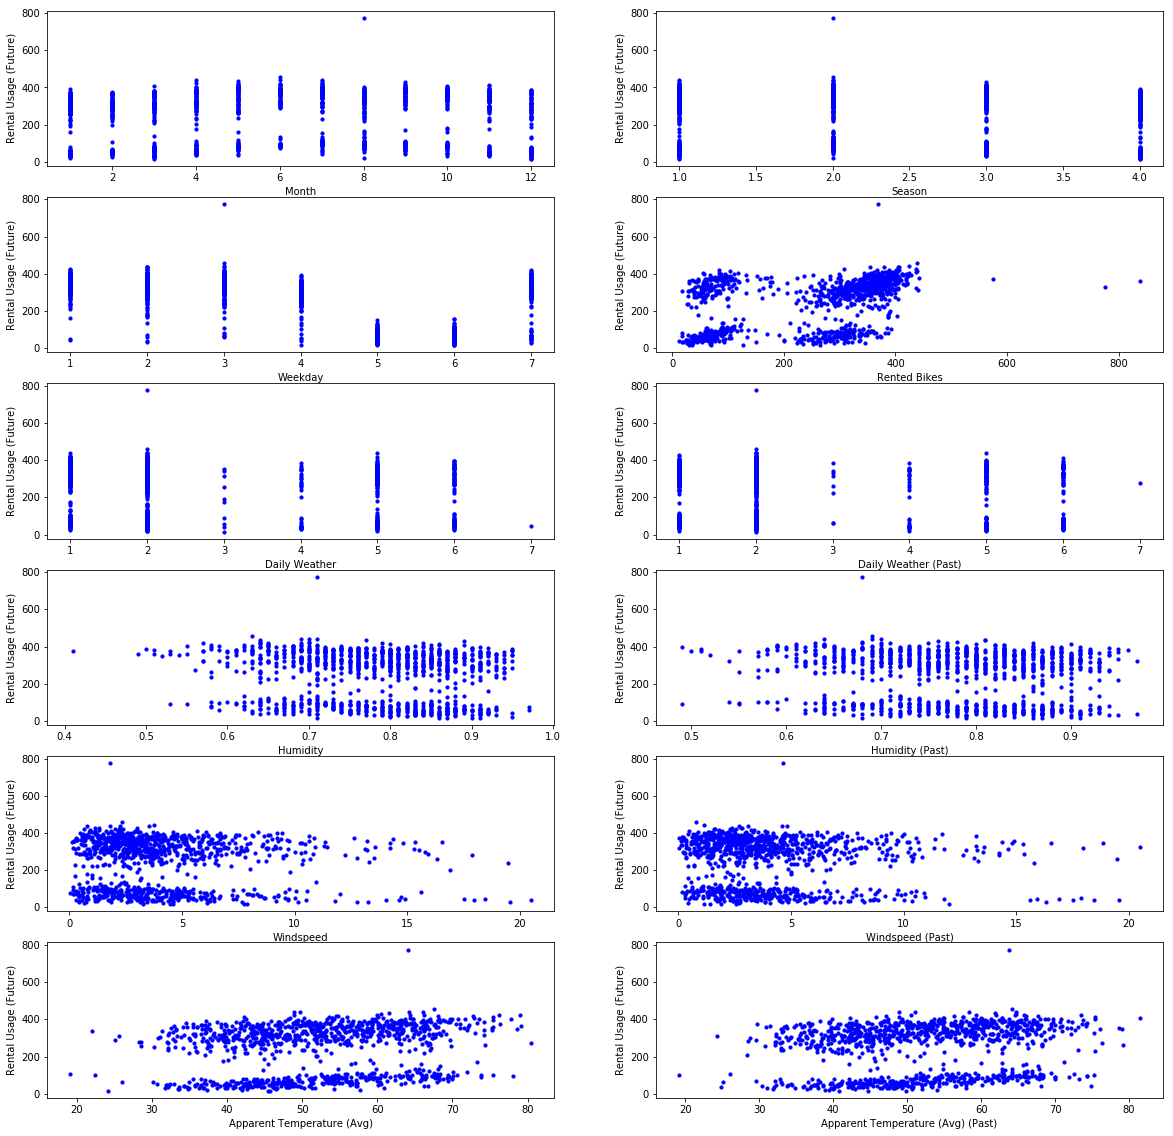
\includegraphics[width=1.4\textwidth]{img/figure9_polynomial_features}\label{fig:figure9_polynomial_features}
\captionof{figure}{Plot of polynomial regression (features)}\label{fig:figure9_polynomial_features}
\end{figure}
\begin{figure}[H]
\hspace{-2.4cm}
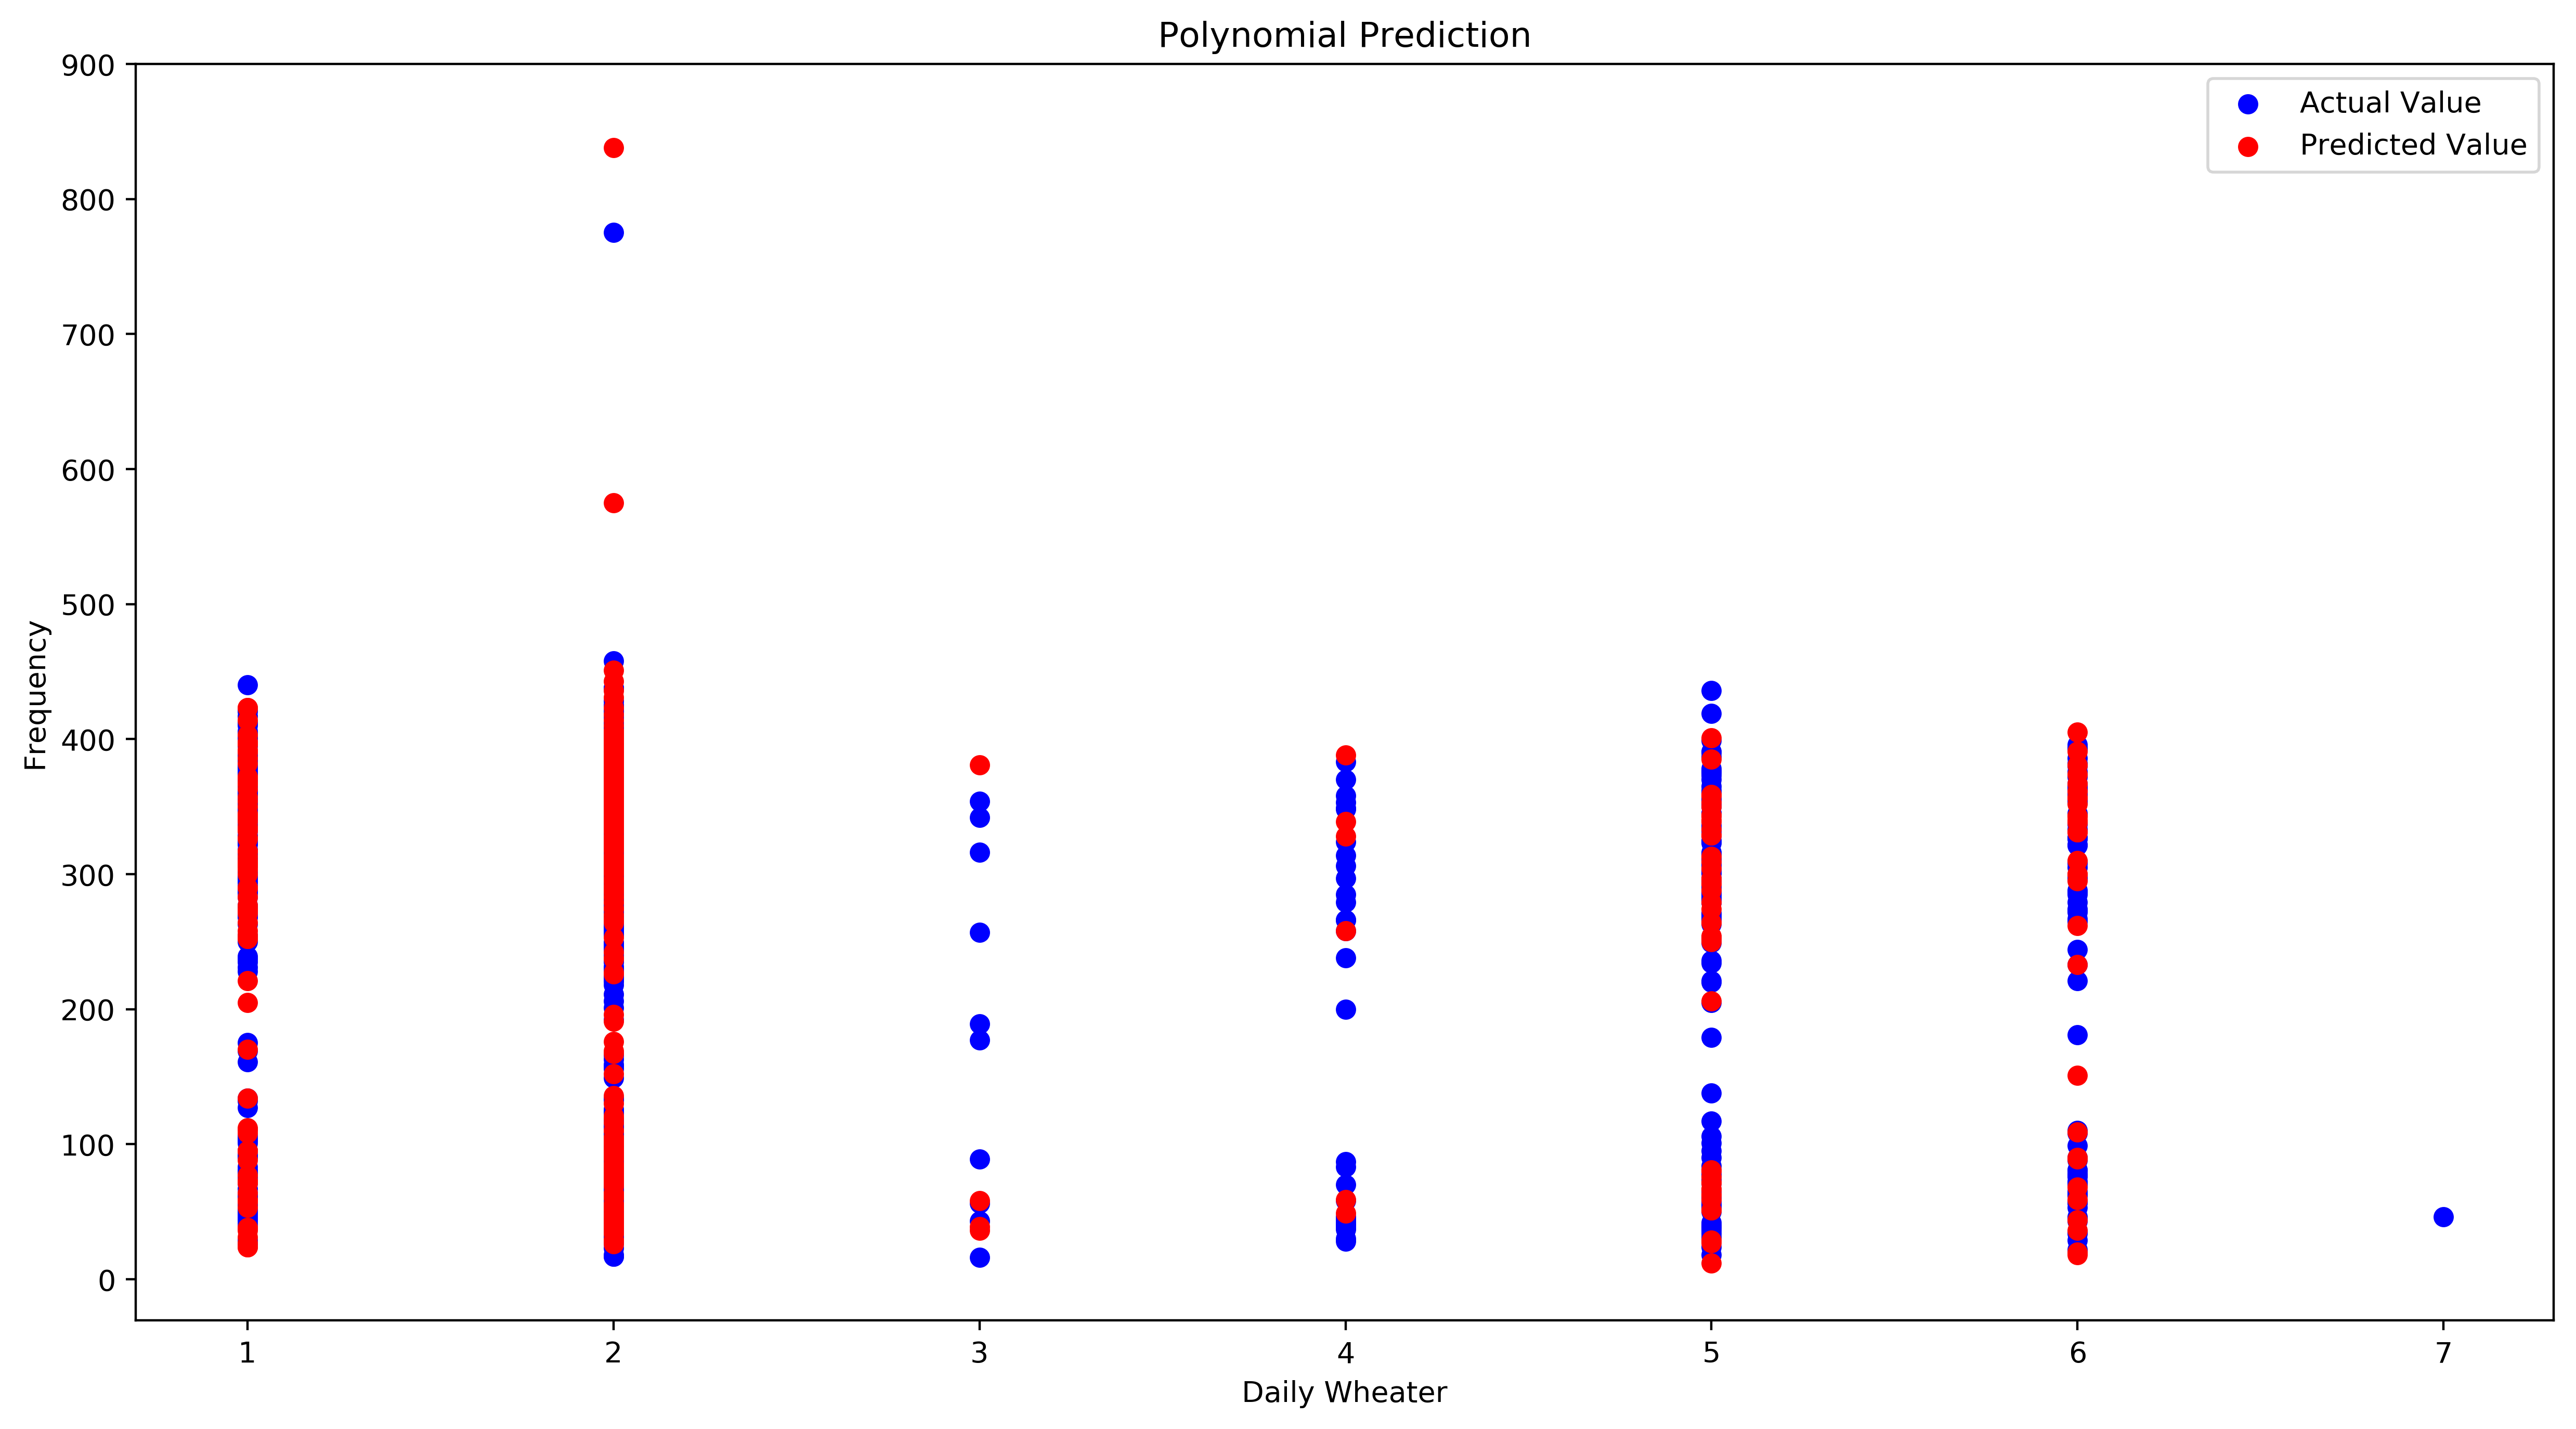
\includegraphics[width=1.3\textwidth]{img/figure10_polynomial_prediction}\label{fig:figure10_polynomial_prediction}
\captionof{figure}{Polynomial Prediction of rental usage on daily weather}\label{fig:figure10_polynomial_prediction}
\end{figure}
% vim:ft=tex

\section{Prediction on Hourly Basis}
\subsection{Introduction}\label{intro_hourly}
Just like in Chapter 3, data prediction is performed with the MLP regressor again. This time, however, the granularity is refined at an hourly level. This makes more training data possible. Furthermore, new correlations are created between the individual features. However, this also requires some changes in the data preparation script. Up to this stage of the project, the aggregation level at day level was sufficient. To be able to format the data from a daily format into an hourly format, both the weather data of the DarkSky API and the cycling usage data have to be re-processed, which is described in more detail in Section 4.1.
Since an hourly data prediction produces much more data than a daily prediction, this user story uses the built up Hadoop cluster as well as PySpark and Zeppelin. The tasks are typical tasks for a cluster-based calculation like Hadoop. Here, too, some parts are reused on the basis of previous scripts (e.g. the generated or calculated weather data).
Section 4.2 deals with the training and prediction of the regression model based on the hourly prepared usage data. Subsequently it is described how the data set can be extended by additional features like "Age" or "local Events". The acquisition of these additional data was carried out by Ankur Mehra project team. 
\subsection{Data Preparation}
Since the long term goal was to predict the usage on a hourly base, some further data
transformation steps are necessary to achieve this goal. Furthermore the data records will
increase significantly on an hourly granularity. Therefore the normal use of Anaconda and Jupyter
on a local computer may be not sufficient due to low physical memory. An ideal use case for our
newly installed Hadoop cluster! There PySpark can be used as already used under Data Profiling
Part 1 in chapter \ref{dp1} to manage \glqq big data\grqq transformations. Unfortunately the behavior and syntax of PySpark
is sometimes a little more complicated than Pandas. For example, in PySpark it is not easily
possible to iterate over rows since the data frame is distributed over the worker nodes and thus it
only allows column wise operations. Moreover, Pandas operations such as „iloc“ are not available
in PySpark. But the API comes also with some advantages, e.g. it is quite performant on big data
scale (i.e. it can easily perform several million of records) and it has an SQL approach.
Functions like \glqq select\grqq \glqq where\grqq and \glqq filter\grqq are syntactical close by to SQL as we know from MySQL
and other database management systems.\\\\
The structure of the weather data is inconsistent due to "hourly weather"  While the other columns
only contain simple values, the column "hourly weather" contains nested JSON lists. This means
that these nested lists must somehow become normal columns. This was a little more complicated
than expected, but not impossible. Fortunately, PySpark allows one to define \glqq schemas\grqq that are
used as a kind of blueprint by Spark to read the Spark data frame. With the following code one
can already create normal columns from the JSON lists:
\begin{figure}[H]
\hspace{-1.6cm}
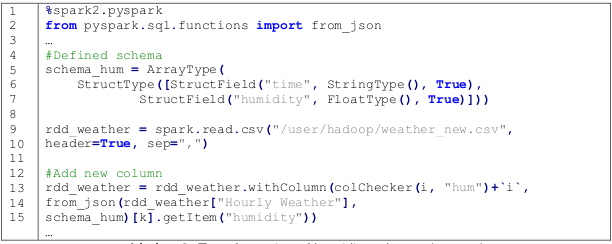
\includegraphics[width=1.2\textwidth]{img/listing5}\label{fig:listing5}
\captionof{figure}{Transformation of humidity columns (excerpt)}\label{fig:listing5}
\end{figure}
he excerpt from \ref{fig:listing5} shows that \glqq structTypes\grqq can be used to search the individual sub lists
of \glqq hourly weather\grqq .
The complete script is contained in the Zeppelin notebook \glqq DFGeneration.json\grqq and can also be found on GitHub.
\\\\
The described transformation creates a new column with the corresponding value for each hour.
The script works dynamically. For example, the user can look at the data with two hours from today,
which then looks like this:
\begin{figure}[H]
\hspace{-1.6cm}
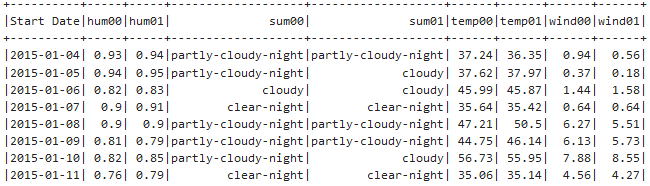
\includegraphics[width=1.2\textwidth]{img/figure7_weather_df}\label{fig:figure7_weather_df}
\captionof{figure}{Weather dataframe after transformation for two hours}\label{fig:figure7_weather_df}
\end{figure}
This (figure \ref{fig:figure7_weather_df}), however, is more like a jumping window technique as it uses days as start date
and not the the single hours on each day. Nevertheless the structure of the data frame from figure \ref{fig:figure7_weather_df} can be used as ground for applying sliding window method.\\\\
However, before the sliding window procedure could be implemented, the \glqq Start Date\grqq from figure \ref{fig:figure7_weather_df} had to be converted to an hourly format, whereby the individual hour columns had to be
combined so that only one \glqq current column\grqq existed. For example, \glqq hum00\grqq and \glqq hum01\grqq should
become something like \glqq Current Humidity\grqq  which shows the humidity value of each hour. This
means that further data preparation steps are necessary.\\\\
First, the exact timestamps of the bicycle data were read in from the provided TfL website and
rounded off to an hourly level. For example, \glqq 23:38\grqq became \glqq 23:00\grqq  Minutes and seconds were
ignored. An arithmetic lap (half-round mode) did not make sense, because then there would be
overlaps with the successor day when 23 o'clock is rounded up. However, this also means that a
slight distortion must be assumed. For example, many bicycles could be rented at a bicycle station
at 17:52 and significantly less after 18 o'clock. Then one would notice a peak at 17 o'clock and a
low usage at 18 o'clock, although in fact more bicycles were rented around 18 o'clock.\\\\
Another problem was that not for every hour there was data about the usage of the bicycle stations.
However, this data quality problem could be solved relatively easy. The missing hours can be
determined by a user defined function. Since every day has 24 hours, this can be calculated
manually as following (figure \ref{fig:listing6}):
\begin{figure}[H]
\hspace{-1.6cm}
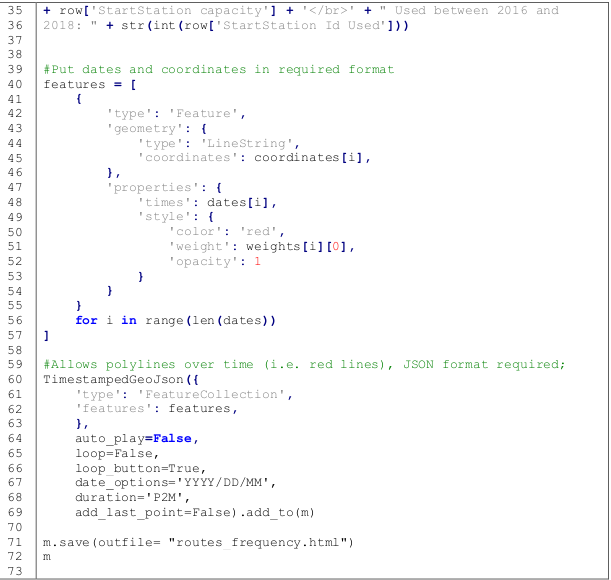
\includegraphics[width=1.2\textwidth]{img/listing2}\label{fig:listing6}
\captionof{figure}{Adding missing hours on usage data}\label{fig:listing6}
\end{figure}
A prerequisite of this method from figure \ref{fig:listing6} is that at least one maximum value and one minimum
value exist that serve as boundaries. If no data was collected on a day at a station, null values
would appear. This does not happen, however, and even if it did, it would be removed at a later
stage as such data does not provide any advantage for training a machine learning model.\\\\
Another problem was how to transform the individual hour columns of the weather data so that
only one column exists instead of e.g. 24 columns, whereby this new column should contain all
values of the 24 columns arranged correctly. Fortunately the function \glqq explode\grqq exists in PySpark
and is provided via the class \glqq pyspark.sql.functions\grqq  With \glqq explode\grqq an array can be passed,
which then returns a new line for each element of the array \cite{RN8}. The corresponding code excerpt
looks as following:
\begin{figure}[H]
\hspace{-1.6cm}
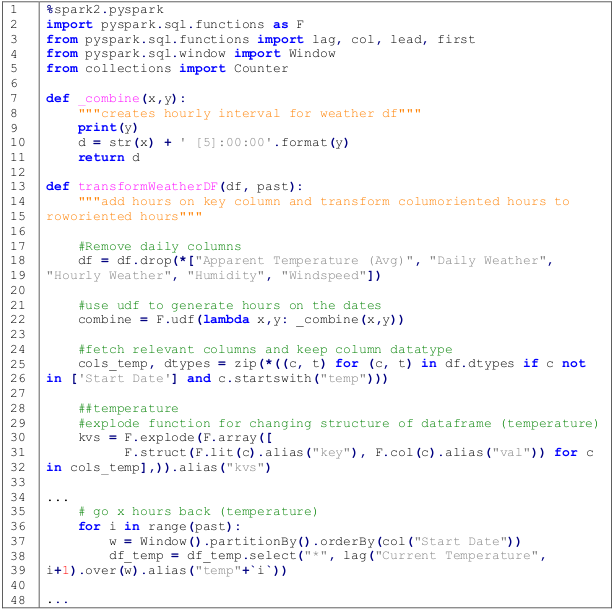
\includegraphics[width=1.2\textwidth]{img/listing7}\label{fig:listing7}
\captionof{figure}{Further transformation of weather data (excerpt)}\label{fig:listing7}
\end{figure}
The code example from figure \ref{fig:listing7} is used to transform the temperature columns, which are
combined into a single column as described above. Thus the weather data frame is prepared to
the extent that every hour of a day belongs to a specific hourly weather value. The lines 35 - 39 show the use of the PySpark function \glqq lag\grqq ,  that over a selected \glqq window\grqq takes the starting
boundary \cite{RN8}. If one increments the index at this point, he will get the previous value from the
window. Depending on how far one wants to go into the past, the window is moved over the data
set and thus a sliding window is achieved. This can also be adapted for the future. With the function
\glqq lead\grqq the ending boundary of a \glqq window\grqq is retrieved \cite{RN8}. Again, the future sliding window is only
applied for the usage (target variable) and not for the weather data or other columns.\\\\
The prepared hourly temperature data with sliding window looks finally as following:
\begin{figure}[H]
\centering
\includegraphics[width=0.8\textwidth]{img/figure8_temperature_df}\label{fig:figure8_temperature_df}
\captionof{figure}{Temperature dataframe after transformation for 3 hours (past)}\label{fig:figure8_temperature_df}
\end{figure}
In this example from figure \ref{fig:figure8_temperature_df} it is clearly recognizable that the initial values contain \glqq null\grqq values, which is due to the fact that no weather data was available before 04.01.2015 (or at least they
were not fetched from Dark Sky). The number of zero values increases with the number of selected
hours into the past. The same applies to the last lines of the Spark data frame, where null values
may be appear for the \glqq future usage\grqq columns. Therefore the first 20 and the last 20 lines of the
data frame are removed at the end.\\\\
With the described PySpark transformations it was possible to create dynamic hourly data frames,
which can then be used in the next step of the modeling phase. A corresponding test file can be
found on GitHub in the folder data preparation.
\subsubsection{Holidays}

To add the bank holidays are day-based, so they should be set on a 24 hour windows.
However, fixing the bank holidays from midnight to midnight the next day might not
be the best solution as people might consider the evening of a bank holiday the same
way as they do for normal week day, while the evening of the day before will be more
interesting. Indeed, when people want to go out in the evening and go to bed late,
they will prefer doing that when they don't have to wake up early in the morning,
thus they may be more likely to use a bike the end of the day before the bank
holiday than of the day itself.

This is why it might be a good idea to test the accuracy of the prediction
placing bank holidays from 6pm the day before to 6pm the day itself.

% TODO: accuracies
% The accuracy of the overall model on the testing data using the bank-holidays
% starting at 6pm is []. When not using this, we get a lower accuracy of
% [].
% TODO: RMSE ?

\subsection{Learning and Prediction}

For the learning part, we used the same algorithm as described in~\ref{data_prediction}.
We trained twenty-four models, one per future hour to predict.
For each model, we only use the past and current data which we match to
the future expected number of rented bike for the given following hour,
no other future data is used.

We used the sliding-windows hourly based data over 48 hours (aggregating per slice
of 6 hours after the first 24 hours).
We have an accuracy of 0.800638 on the test dataset.
On the graph below, you can see several randomly selected days in the testing set
starting at midnight and predicting for the whole day. The title above each graph
indicates the date displayed, the actual expected value is in red and the
predicted one is in blue.
\begin{figure}[H]
\hspace{-0.9cm}
\includegraphics[width=1.1\textwidth]{img/hourly_predictions}
\captionof{figure}{Comparison of expected (red) and predicted (blue) hourly rented bikes on test dataset}\label{fig:hourly_pred}
\end{figure}

As we can see on the Figure~\ref{fig:hourly_pred} and considering the measured accuracy,
we can see that we can predict quite well the amount of rented bikes for the following
24 hours based on the data of the previous 48 hours.

\chapter{Postal Code Database (Junior)}
% TODO: other things ?
% vim:ft=tex

\section{Task Description}

% vim:ft=tex

\section{Conclusion}


\newpage
\bibliographystyle{plain}
\bibliography{./bibtex/library}
\renewcommand{\listfigurename}{B Illustration Directory}
\listoffigures
\section*{C List of Abbreviations}
\addcontentsline{toc}{section}{C List of Abbreviations}
\begin{acronym}
    \acro{yarn}[YARN]{Yet Another Resource Negotiator}
    \acro{sql} [SQL]{Structured Query Language}
    \acro{nsql} [NoSQL]{Not only Sql}
    \acro{pl}[PL/pgSQL] {Procedural Language/PostgreSQL}
    \acro{osm}[OSM]{OpenStreetMap}
    \acro{hdp}[HDP]{Hortonworks Data Platform}
    \acro{hdfs} [HDFS]{Hadoop Distributed File System}
    \acro{osm}[OSM]{OpenStreetMap}
    \acro{dfsio}[DFSIO]{Data File System I/O}
    \acro{mlp}[MLPRegressor]{Multi-layer Perceptron Regressor}
    \acro{rmse}[RMSE]{Root Mean Square Error}
\end{acronym}
\newpage
\section*{D Attachments}
\addcontentsline{toc}{section}{D Attachments}
\subsection*{Attachment 1:\\ Responsibilities}\label{resp}
\begin{landscape}
    \begin{table}[]
        \begin{tabular}{l|l|l|l|}
            \cline{2-4}
                                & Sprint 1                                                                                                                                                                                                                                          & Sprint 2                                                                                                                                                                                                                                                                                    & Sprint 3                                                                                                                                                                                                                                           \\ \hline
            \multicolumn{1}{|l|}{Anass}     & \begin{tabular}[c]{@{}l@{}}hadoop docu\\ creation of users in hadoop\\ install nominatim/ components\\ import planet database\\ compute postcodes\\ reverse geocoding in bulk\end{tabular}                                                        & \begin{tabular}[c]{@{}l@{}}design big picture\\ research maps for WebApp\\ research Django\end{tabular}                                                                                                                                                                                     & \begin{tabular}[c]{@{}l@{}}Fixing dead hadoop node\\ installGraphhopper\\ docu Graphhopper\\ import OSM data to Graphhopper\\ write report part of edited tasks\end{tabular}                                                                       \\ \hline
            \multicolumn{1}{|l|}{Guillaume} & \begin{tabular}[c]{@{}l@{}}create user for nominatim\\ uploading SSH keys\\ querying centroids\\ distances by route\\ distances in bulk\end{tabular}                                                                                              & \begin{tabular}[c]{@{}l@{}}create GitHub repos\\ unioned all notebooks\\ connect geopy with nominatim\\ reserach Django\\ Django tutorial\\ script for initializing database\\ initialize db with postcodes\end{tabular}                                                                    & \begin{tabular}[c]{@{}l@{}}research postcodes in PostgresDB\\ script for filling zipcodes in db\\ write report part of edited tasks\end{tabular}                                                                                                   \\ \hline
            \multicolumn{1}{|l|}{Kathi}     & \begin{tabular}[c]{@{}l@{}}creating team Box\\ creating templates\\ documentation OSM API\\ geocoding/reverse Geocoding\\ distances as the crow flies\\ design ER model\\ create presentation for sprint review\\ Scrum Master tasks\end{tabular} & \begin{tabular}[c]{@{}l@{}}design \& finalize Big Picture\\ Graphhopper docu \& example\\ install x2go server\\ docu access vms via x2go client\\ define mockup structure\\ create mockup\\ install mysql database\\ create presentation for sprint review\\ Scrum Master tasks\end{tabular} & \begin{tabular}[c]{@{}l@{}}latex template for project report\\ write report part of edited tasks\\ union texts of team members to report\\ reorganize GitHub repositories\\ create presentation for sprint review\\ Scrum Master tasks\end{tabular} \\ \hline
            \multicolumn{1}{|l|}{Pascal}    & \begin{tabular}[c]{@{}l@{}}research hadoop distributions\\ find weightened comparison data\\ hadoop documentation\\ Installation of HDP\\ Implement Map Reduce Job\end{tabular}                                                                    & \begin{tabular}[c]{@{}l@{}}Solving Hadoop issues\\ collect TFL data \& \\ data munging on Hadoop\\ create mockup\\ installed Django server\end{tabular}                                                                                                                                     & \begin{tabular}[c]{@{}l@{}}create spark file sizing notebook\\ CycleRoutes prepared \& collected \\ plotting statistics of cycle usage\\ solving hadoop errors\\ plotting routes of cycle data\\ write report part of edited tasks\end{tabular}    \\ \hline
        \end{tabular}
        \end{table}
        \end{landscape}
            \end{document}
